% Problems, Chapter 3: Boundary-Value Problems in Electrostatics: II
% Jackson, Classical Electrodynamics, 3rd ed.
% Requires: amsmath, amssymb, tikz

\section*{Problems}

\Needspace{5\baselineskip}
\par\bigskip
\noindent\textbf{3.1}\quad Two concentric spheres have radii $a$, $b$ ($b>a$) and each is divided into two hemispheres by the same horizontal plane. The upper hemisphere of the inner sphere and the lower hemisphere of the outer sphere are maintained at potential $V$. The other hemispheres are at zero potential.

Determine the potential in the region $a\leq r\leq b$ as a series in Legendre polynomials. Include terms at least up to $l=4$. Check your solution against known results in the limiting cases $b\to\infty$, and $a\to0$.
\solution

Put $\mu=\cos\theta$ and expand the boundary values as
$V_a(\mu)=\sum_l v_lP_l(\mu)$ and $V_b(\mu)=\sum_l w_lP_l(\mu)$.
Orthogonality gives
\[
v_l=\frac{(2l+1)V}{2}\int_0^1P_l(u)\,du,\qquad
w_l=(-1)^lv_l.
\]
For $l\geq1$, integrate
$(2l+1)P_l=(P_{l+1}-P_{l-1})'$ to obtain
\[
v_l=\frac V2[P_{l-1}(0)-P_{l+1}(0)].
\]
Thus $v_0=V/2$, $v_1=3V/4$, $v_3=-7V/16$, and all even
$l>0$ coefficients vanish.  For each angular order, Laplace's
equation gives $f_l(r)=\alpha_lr^l+\beta_lr^{-l-1}$.  The two
boundary equations, after multiplication by $a^{l+1}$ and $b^{l+1}$,
are
\[
\alpha_la^{2l+1}+\beta_l=a^{l+1}v_l,\qquad
\alpha_lb^{2l+1}+\beta_l=b^{l+1}w_l.
\]
Writing $D_l=b^{2l+1}-a^{2l+1}$, subtraction and back-substitution give
\[
\alpha_l=\frac{b^{l+1}w_l-a^{l+1}v_l}{D_l},\qquad
\beta_l=\frac{a^{l+1}b^{2l+1}v_l-b^{l+1}a^{2l+1}w_l}{D_l}.
\]
Thus $f_l=v_lA_l+w_lB_l$, where the two radial interpolants are
\[
A_l(r)=\frac{a^{l+1}(b^{2l+1}-r^{2l+1})}
 {r^{l+1}(b^{2l+1}-a^{2l+1})},\qquad
B_l(r)=\frac{b^{l+1}(r^{2l+1}-a^{2l+1})}
 {r^{l+1}(b^{2l+1}-a^{2l+1})}.
\]
Each is a linear combination of $r^l$ and $r^{-l-1}$, and
$(A_l(a),A_l(b))=(1,0)$, $(B_l(a),B_l(b))=(0,1)$.
Consequently
\[
\boxed{\Phi=\frac V2+
\sum_{\substack{l\geq1\\l\ \mathrm{odd}}}
\frac V2[P_{l-1}(0)-P_{l+1}(0)]
[A_l(r)-B_l(r)]P_l(\mu).}
\]
Through $l=4$ this is
\[
\Phi=\frac V2+\frac{3V}{4}(A_1-B_1)\mu
-\frac{7V}{16}(A_3-B_3)\frac{5\mu^3-3\mu}{2}
+\text{terms with }l\geq5.
\]
The $l=0$ contribution is constant because $A_0+B_0=1$.
At a boundary jump the Legendre series takes the mean value $V/2$.

For fixed $a,r$, $b\to\infty$ gives $A_l\to(a/r)^{l+1}$ and
$B_l\to0$ for $l>0$.  The limit is therefore the exterior hemispherical
solution with asymptotic potential $V/2$; the distant outer boundary
retains this constant offset.  In the limit $a\to0$ at fixed $r,b$,
$A_l\to0$ and $B_l\to(r/b)^l$ for $l>0$, giving the regular interior
solution with the lower hemisphere of the sphere at $V$.

\Needspace{5\baselineskip}
\par\bigskip
\noindent\textbf{3.2}\quad A spherical surface of radius $R$ has charge uniformly distributed over its surface with a density $Q/4\pi R^{2}$, except for a spherical cap at the north pole, defined by the cone $\theta=\alpha$.
\begin{enumerate}
\item[(a)] Show that the potential inside the spherical surface can be expressed as
\[
\Phi=\frac{Q}{8\pi\epsilon_{0}}\sum_{l=0}^{\infty}\frac{1}{2l+1}\left[P_{l+1}(\cos\alpha)-P_{l-1}(\cos\alpha)\right]\frac{r^{l}}{R^{l+1}}P_{l}(\cos\theta)
\]
where, for $l=0$, $P_{l-1}(\cos\alpha)=-1$. What is the potential outside?
\item[(b)] Find the magnitude and the direction of the electric field at the origin.
\item[(c)] Discuss the limiting forms of the potential (part a) and electric field (part b) as the spherical cap becomes (1) very small, and (2) so large that the area with charge on it becomes a very small cap at the south pole.
\end{enumerate}
\solution

Write $c=\cos\alpha$; the charged portion is $-1\leq\mu'\leq c$.
The symbol $Q$ specifies the original full-sphere density: the charge
actually present is $Q_{\rm rem}=Q(1+c)/2$.
Averaging the Coulomb expansion over the source azimuth gives
\[
\int_0^{2\pi}P_l(\cos\gamma)\,d\phi'
=2\pi P_l(\mu)P_l(\mu').
\]
\textbf{(a)} Hence
\[
\Phi=\frac{Q}{8\pi\epsilon_0}
\sum_{l=0}^\infty P_l(\mu)\frac{r_<^l}{r_>^{l+1}}
\int_{-1}^cP_l(u)\,du,
\quad r_<=\min(r,R),\quad r_>=\max(r,R).
\]
For $l\geq1$ the integral is
$[P_{l+1}(c)-P_{l-1}(c)]/(2l+1)$ because the lower-end terms cancel.
For $l=0$ it is $1+c$, reproduced by the stipulated $P_{-1}=-1$.
This proves the displayed interior expression.  The exterior expression
is the same sum with $r^l/R^{l+1}$ replaced by $R^l/r^{l+1}$.
Continuity at $r=R$ follows term by term; its radial derivative has the
jump $\partial_r\Phi_{\rm out}-\partial_r\Phi_{\rm in}=-\sigma/\epsilon_0$.

\textbf{(b)} Only $l=1$ contributes to the gradient at the origin.
Since $P_2(c)-P_0(c)=-3(1-c^2)/2$,
\[
\Phi=\frac{Q(1+c)}{8\pi\epsilon_0R}
-\frac{Q\sin^2\alpha}{16\pi\epsilon_0R^2}z+O(r^2),\qquad
\boxed{\mathbf E(0)=\frac{Q\sin^2\alpha}{16\pi\epsilon_0R^2}\,\hat{\mathbf z}.}
\]
For positive $Q$ the field points toward the missing north cap; reversing
$Q$ reverses its direction.

\textbf{(c)} For $\alpha\ll1$, the missing charge is
$\delta Q=Q(1-c)/2=Q\alpha^2/4+O(\alpha^4)$.
Away from the shrinking cap its potential is that of a point charge at
$R\hat{\mathbf z}$ to leading order.  Thus
\[
\Phi=\frac{Q}{4\pi\epsilon_0\max(r,R)}
-\frac{Q\alpha^2}{16\pi\epsilon_0|\mathbf r-R\hat{\mathbf z}|}
+O(\alpha^4),\qquad
\mathbf E(0)=\frac{Q\alpha^2}{16\pi\epsilon_0R^2}\hat{\mathbf z}
+O(\alpha^4).
\]
For $\beta=\pi-\alpha\ll1$, only the south cap remains, with
$Q_{\rm rem}=Q\beta^2/4+O(\beta^4)$, and
\[
\Phi=\frac{Q\beta^2}{16\pi\epsilon_0|\mathbf r+R\hat{\mathbf z}|}
+O(\beta^4),\qquad
\mathbf E(0)=\frac{Q\beta^2}{16\pi\epsilon_0R^2}\hat{\mathbf z}
+O(\beta^4).
\]
These expansions are not uniform at the cap itself.  With the specified
fixed density the remaining charge and field tend to zero; if instead
its total charge is held fixed, the south-cap limit is an ordinary
point charge of that fixed magnitude.

\Needspace{5\baselineskip}
\par\bigskip
\noindent\textbf{3.3}\quad A thin, flat, conducting, circular disc of radius $R$ is located in the $x$-$y$ plane with its center at the origin, and is maintained at a fixed potential $V$. With the information that the charge density on a disc at fixed potential is proportional to $(R^{2}-\rho^{2})^{-1/2}$, where $\rho$ is the distance out from the center of the disc,
\begin{enumerate}
\item[(a)] show that for $r>R$ the potential is
\[
\Phi(r,\theta,\phi)=\frac{2V}{\pi}\frac{R}{r}\sum_{l=0}^{\infty}\frac{(-1)^{l}}{2l+1}\left(\frac{R}{r}\right)^{2l}P_{2l}(\cos\theta)
\]
\item[(b)] find the potential for $r<R$.
\item[(c)] What is the capacitance of the disc?
\end{enumerate}
\solution

Let $\sigma(\rho)=C_0/\sqrt{R^2-\rho^2}$ denote the total sheet
charge density, including both faces.  At the center,
\[
V=\frac{1}{4\pi\epsilon_0}\int_0^R
\frac{2\pi\rho\,C_0\,d\rho}{\rho\sqrt{R^2-\rho^2}}
=\frac{\pi C_0}{4\epsilon_0},
\quad C_0=\frac{4\epsilon_0V}{\pi}.
\]
\textbf{(a)} The azimuthal average of the Coulomb expansion yields
\[
\Phi=\frac{C_0}{2\epsilon_0}
\sum_{n=0}^\infty\frac{P_{2n}(0)P_{2n}(\cos\theta)}{r^{2n+1}}
\int_0^R\frac{\rho^{2n+1}\,d\rho}{\sqrt{R^2-\rho^2}}.
\]
Odd orders vanish.  With $t=\rho^2/R^2$ the integral equals
\[
\frac{R^{2n+1}}2 B(n+1,\tfrac12)
=R^{2n+1}\frac{2^{2n}(n!)^2}{(2n+1)!}.
\]
Multiplication by $P_{2n}(0)=(-1)^n(2n)!/[2^{2n}(n!)^2]$
gives $(-1)^nR^{2n+1}/(2n+1)$ and hence the required series.

\textbf{(b)} First compute the potential on the positive axis:
\[
\Phi(0,z)=\frac{2V}{\pi}\int_0^R
\frac{\rho\,d\rho}{\sqrt{R^2-\rho^2}\sqrt{\rho^2+z^2}}
=\frac{2V}{\pi}\tan^{-1}\frac Rz
=V-\frac{2V}{\pi}\tan^{-1}\frac zR.
\]
For example, $u=\sqrt{R^2-\rho^2}$ changes the integral to
$\int_0^Rdu/\sqrt{R^2+z^2-u^2}$, giving the stated inverse tangent.
In the upper half-ball expand the last expression in powers of $z/R$.
The unique regular, axially symmetric harmonic extension of $z^l$ is
$r^lP_l(\cos\theta)$.  Reflection in the disc then gives
\[
\boxed{\Phi=V-\frac{2V}{\pi}\sum_{n=0}^\infty
\frac{(-1)^n}{2n+1}\left(\frac rR\right)^{2n+1}
P_{2n+1}(|\cos\theta|),\qquad r<R.}
\]
On the disc all odd Legendre polynomials vanish at zero, so $\Phi=V$.
The absolute value is essential: there is a normal-derivative jump at
the charged sheet and no single harmonic power series through it.

\textbf{(c)} Integration of the sheet density gives
\[
Q=2\pi C_0\int_0^R\frac{\rho\,d\rho}{\sqrt{R^2-\rho^2}}
=8\epsilon_0RV,\qquad \boxed{C=8\epsilon_0R.}
\]
The exterior monopole term is correspondingly $Q/(4\pi\epsilon_0r)$.

\Needspace{5\baselineskip}
\par\bigskip
\noindent\textbf{3.4}\quad The surface of a hollow conducting sphere of inner radius $a$ is divided into an \emph{even number} of equal segments by a set of planes; their common line of intersection is the $z$ axis and they are distributed uniformly in the angle $\phi$. (The segments are like the skin on wedges of an apple, or the earth's surface between successive meridians of longitude.) The segments are kept at fixed potentials $\pm V$, alternately.
\begin{enumerate}
\item[(a)] Set up a series representation for the potential inside the sphere for the general case of $2n$ segments, and carry the calculation of the coefficients in the series far enough to determine exactly which coefficients are different from zero. For the nonvanishing terms, exhibit the coefficients as an integral over $\cos\theta$.
\item[(b)] For the special case of $n=1$ (two hemispheres) determine explicitly the potential up to and including all terms with $l=3$. By a coordinate transformation verify that this reduces to result (3.36) of Section 3.3.
\end{enumerate}
\solution

Choose the angular origin so that the boundary value is
$V\,\operatorname{sgn}[\sin(n\phi)]$.  A rotation about $z$ covers any
other placement of the segments.  Its Fourier series is
\[
V(\phi)=\frac{4V}{\pi}\sum_{s=0}^\infty
\frac{\sin(m_s\phi)}{2s+1},\qquad m_s=(2s+1)n.
\]
\textbf{(a)} Use real associated Legendre functions with the
Condon--Shortley phase, $P_l^m=(-1)^m(1-u^2)^{m/2}d^mP_l/du^m$,
as in Jackson's Eq.~(3.49), p.~108.  Consequently
$Y_{lm}=[(2l+1)(l-m)!/(4\pi(l+m)!)]^{1/2}P_l^m e^{im\phi}$
has no additional phase [Eq.~(3.53)].
The regular solution and its coefficients are
\begin{align*}
\Phi&=\sum_{s=0}^\infty\sum_{l=m_s}^\infty
c_{lm_s}(r/a)^lP_l^{m_s}(\cos\theta)\sin(m_s\phi),\\
c_{lm}&=\frac{2V(2l+1)}{\pi(2s+1)}
\frac{(l-m)!}{(l+m)!}\int_{-1}^1P_l^m(u)\,du,
\qquad m=(2s+1)n.
\end{align*}
Here the factor $(2l+1)(l-m)!/[2(l+m)!]$ is the inverse
associated-Legendre norm.  All cosine modes, $m=0$ modes, and all
other azimuthal orders vanish.  Parity gives
$P_l^m(-u)=(-1)^{l+m}P_l^m(u)$, so $l+m$ must be even.
To prove that there are no further zeros, put
$I_{lm}=\int_{-1}^1P_l^m(u)\,du$.  The associated-Legendre identities
\[
(1-u^2)(P_l^m)'=-luP_l^m+(l+m)P_{l-1}^m,\qquad
(2l+1)uP_l^m=(l-m+1)P_{l+1}^m+(l+m)P_{l-1}^m
\]
give, after integration by parts in the first identity,
\[
(l+2)\int_{-1}^1uP_l^m\,du=(l+m)I_{l-1,m},\qquad
I_{l+1,m}=\frac{(l-1)(l+m)}{(l+2)(l-m+1)}I_{l-1,m}.
\]
The boundary term vanishes because $(1-u^2)P_l^m\to0$.  Relabeling
$l=L+1$ yields
\[
I_{L+2,m}=\frac{L(L+m+1)}{(L+3)(L-m+2)}I_{L,m}.
\]
The starting value follows from
$P_m^m=(-1)^m(2m-1)!!(1-u^2)^{m/2}$:
\[
I_{mm}=(-1)^m(2m-1)!!\,B(1/2,1+m/2)\ne0.
\]
Every multiplier in the recurrence is positive for $L\geq m\geq1$;
hence every $l=m,m+2,\ldots$ survives.  Iterating the recurrence
and using $\Gamma(x+1)=x\Gamma(x)$ also gives the closed form
\[
\int_{-1}^1P_l^m(u)\,du
=(-1)^m2^{m-1}m\,
\frac{\Gamma(l/2)\Gamma((l+m+1)/2)}
{\Gamma((l-m+2)/2)\Gamma((l+3)/2)},
\]
whose gamma factors are finite and positive.  This also specifies
unambiguously which coefficients in the integral formula survive.

\textbf{(b)} For $n=1$, the required integrals are
\[
\int P_1^1\,du=-\frac\pi2,\qquad
\int P_3^1\,du=-\frac{3\pi}{16},\qquad
\int P_3^3\,du=-\frac{45\pi}{8},
\]
where all integrals run from $-1$ to $1$.  Therefore, through $l=3$,
\[
\Phi=-\frac{3V}{2}\frac ra P_1^1(\cos\theta)\sin\phi
-\left(\frac ra\right)^3
\left[\frac{7V}{32}P_3^1(\cos\theta)\sin\phi
+\frac{7V}{192}P_3^3(\cos\theta)\sin3\phi\right]+O((r/a)^5).
\]
The new polar axis may be chosen along $+y$, so
$\cos\Theta=y/r=\sin\theta\sin\phi$.  Substitution of
$P_1^1=-\sin\theta$,
$P_3^1=-\tfrac32(5\cos^2\theta-1)\sin\theta$, and
$P_3^3=-15\sin^3\theta$, with
$\sin3\phi=3\sin\phi-4\sin^3\phi$, reduces this to
\[
\Phi=V\left[\frac32\frac ra P_1(\cos\Theta)
-\frac78\left(\frac ra\right)^3P_3(\cos\Theta)\right]
+O((r/a)^5),
\]
which is Eq.~(3.36) in the rotated coordinates.

\Needspace{5\baselineskip}
\par\bigskip
\noindent\textbf{3.5}\quad A hollow sphere of inner radius $a$ has the potential specified on its surface to be $\Phi=V(\theta,\phi)$. Prove the equivalence of the two forms of solution for the potential inside the sphere:
\begin{enumerate}
\item[(a)] $\displaystyle\Phi(\mathbf{x})=\frac{a(a^{2}-r^{2})}{4\pi}\int\frac{V(\theta',\phi')}{(r^{2}+a^{2}-2ar\cos\gamma)^{3/2}}\;d\Omega'$

where $\cos\gamma=\cos\theta\cos\theta'+\sin\theta\sin\theta'\cos(\phi-\phi')$.
\item[(b)] $\displaystyle\Phi(\mathbf{x})=\sum_{l=0}^{\infty}\sum_{m=-l}^{l}A_{lm}\left(\frac{r}{a}\right)^{l}Y_{lm}(\theta,\phi)$

where $A_{lm}=\int d\Omega'\;Y_{lm}^{*}(\theta',\phi')V(\theta',\phi')$.
\end{enumerate}
\solution

Let $t=r/a<1$ and $u=\cos\gamma$.  The Legendre generating function is
$F(t,u)=(1-2tu+t^2)^{-1/2}=\sum_{l\geq0}t^lP_l(u)$.
Differentiate within its convergent power series:
\[
F+2t\partial_tF
=\frac{1-t^2}{(1-2tu+t^2)^{3/2}}
=\sum_{l=0}^\infty(2l+1)t^lP_l(u).
\]
Consequently the kernel in (a) is
\[
\frac{a(a^2-r^2)}{4\pi(a^2+r^2-2ar\cos\gamma)^{3/2}}
=\sum_{l=0}^\infty\frac{2l+1}{4\pi}
(r/a)^lP_l(\cos\gamma).
\]
Use the addition theorem
\[
\frac{2l+1}{4\pi}P_l(\cos\gamma)
=\sum_{m=-l}^lY_{lm}(\theta,\phi)Y_{lm}^*(\theta',\phi').
\]
Inserting it into (a), interchanging the integral and the uniformly
convergent series on any closed ball $r\leq r_0<a$, and grouping the
source integral gives exactly (b) with its stated $A_{lm}$.
Conversely, insert those coefficients into (b) and sum the same kernel
to recover (a).  For an integrable boundary value this proves the
interior equivalence; for continuous boundary data the limiting
Poisson integral takes the assigned surface value.  Constant data
provide a normalization check: only $l=0$ remains and $\Phi=V$.

\Needspace{5\baselineskip}
\par\bigskip
\noindent\textbf{3.6}\quad Two point charges $q$ and $-q$ are located on the $z$ axis at $z=+a$ and $z=-a$, respectively.
\begin{enumerate}
\item[(a)] Find the electrostatic potential as an expansion in spherical harmonics and powers of $r$ for both $r>a$ and $r<a$.
\item[(b)] Keeping the product $qa\equiv p/2$ constant, take the limit of $a\to0$ and find the potential for $r\neq0$. This is by definition a dipole along the $z$ axis and its potential.
\item[(c)] Suppose now that the dipole of part b is surrounded by a \emph{grounded} spherical shell of radius $b$ concentric with the origin. By linear superposition find the potential everywhere inside the shell.
\end{enumerate}
\solution

\textbf{(a)} The direct potential is
\[
\Phi=\frac{q}{4\pi\epsilon_0}
\left(\frac1{|\mathbf r-a\hat{\mathbf z}|}
-\frac1{|\mathbf r+a\hat{\mathbf z}|}\right).
\]
In the Coulomb expansion the two source directions contribute
$P_l(\cos\theta)$ and $P_l(-\cos\theta)=(-1)^lP_l(\cos\theta)$.
Even orders cancel, giving
\[
\boxed{\Phi=\frac{q}{2\pi\epsilon_0}
\sum_{j=0}^\infty P_{2j+1}(\cos\theta)
\begin{cases}
a^{2j+1}/r^{2j+2},&r>a,\\
r^{2j+1}/a^{2j+2},&r<a.
\end{cases}}
\]
This is a spherical-harmonic expansion because
$P_l(\cos\theta)=\sqrt{4\pi/(2l+1)}Y_{l0}$; all $m\ne0$
coefficients vanish.  The source points themselves are excluded.

\textbf{(b)} With $2qa=p$ fixed, the $l=1$ coefficient remains
finite and every higher term has an extra factor $a^{2j}$.  At each
fixed $r>0$,
\[
\boxed{\Phi_{\rm dip}=\frac{p\cos\theta}{4\pi\epsilon_0r^2}.}
\]

\textbf{(c)} A regular $l=1$ harmonic $Ar\cos\theta$ can cancel
the dipole's surface value.  The equation
$p/(4\pi\epsilon_0b^2)+Ab=0$ fixes $A=-p/(4\pi\epsilon_0b^3)$.
Thus
\[
\boxed{\Phi=\frac{p\cos\theta}{4\pi\epsilon_0}
\left(\frac1{r^2}-\frac r{b^3}\right),\qquad0<r<b.}
\]
The added field is the uniform field
$+p\hat{\mathbf z}/(4\pi\epsilon_0b^3)$; it is regular at the
source and makes the total potential vanish at $r=b$.

\Needspace{5\baselineskip}
\par\bigskip
\noindent\textbf{3.7}\quad Three point charges ($q$, $-2q$, $q$) are located in a straight line with separation $a$ and with the middle charge ($-2q$) at the origin of a grounded conducting spherical shell of radius $b$, as indicated in the sketch.

\begin{center}
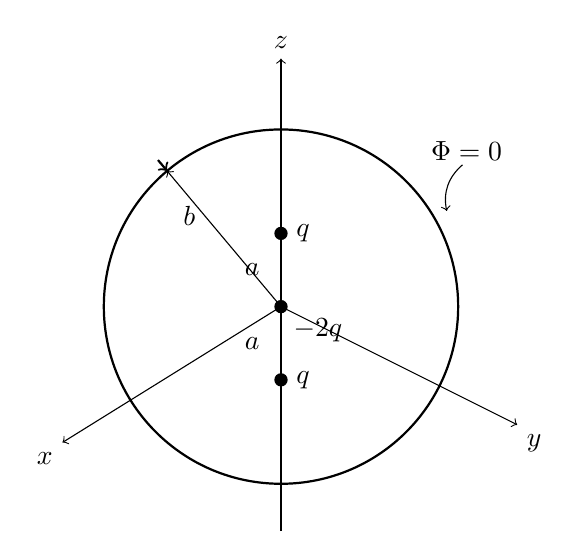
\begin{tikzpicture}[scale=1.5]
  % grounded sphere
  \draw[thick] (0,0) circle (1.5);
  % axes
  \draw[->] (0,-1.9) -- (0,2.1) node[above] {$z$};
  \draw[->] (0,0) -- (-1.85,-1.15) node[below left] {$x$};
  \draw[->] (0,0) -- (2.0,-1.0) node[below right] {$y$};
  % radius b arrow
  \draw[<-,thick] (130:1.5) -- (130:1.62);
  \draw[->] (0,0) -- (130:1.5);
  \node[left] at (130:1.0) {$b$};
  % charges on z axis
  \fill (0,0.62) circle (1.6pt) node[right=2pt] {$q$};
  \fill (0,0) circle (1.6pt) node[below right=1pt] {$-2q$};
  \fill (0,-0.62) circle (1.6pt) node[right=2pt] {$q$};
  % separation labels
  \node[left] at (-0.1,0.31) {$a$};
  \node[left] at (-0.1,-0.31) {$a$};
  % Phi = 0 with pointer to sphere
  \node at (40:2.05) {$\Phi=0$};
  \draw[->] (38:1.95) to[bend right] (30:1.62);
\end{tikzpicture}
\par\vspace{0.5em}\textbf{Problem 3.7}
\end{center}

\begin{enumerate}
\item[(a)] Write down the potential of the three charges in the absence of the grounded sphere. Find the limiting form of the potential as $a\to0$, but the product $qa^{2}=Q$ remains finite. Write this latter answer in spherical coordinates.
\item[(b)] The presence of the grounded sphere of radius $b$ alters the potential for $r<b$. The added potential can be viewed as caused by the surface-charge density induced on the inner surface at $r=b$ or by image charges located at $r>b$. Use linear superposition to satisfy the boundary conditions and find the potential everywhere inside the sphere for $r<a$ and $r>a$. Show that in the limit $a\to0$,
\[
\Phi(r,\theta,\phi)\to\frac{Q}{2\pi\epsilon_{0}r^{3}}\left(1-\frac{r^{5}}{b^{5}}\right)P_{2}(\cos\theta)
\]
\end{enumerate}
\solution

\textbf{(a)} Before inserting the conductor,
\[
\Phi_{\rm free}=\frac{q}{4\pi\epsilon_0}
\left(\frac1{\sqrt{r^2+a^2-2ar\cos\theta}}
+\frac1{\sqrt{r^2+a^2+2ar\cos\theta}}-\frac2r\right).
\]
For $r>a$ the $l=0$ terms cancel and odd terms cancel by reflection:
\[
\Phi_{\rm free}=\frac{q}{2\pi\epsilon_0}
\sum_{j=1}^\infty\frac{a^{2j}}{r^{2j+1}}P_{2j}(\cos\theta).
\]
Therefore, for fixed $r>0$ and $qa^2=Q$,
\[
\Phi_{\rm free}\longrightarrow
\frac{Q}{2\pi\epsilon_0r^3}P_2(\cos\theta)
=\frac{Q(3\cos^2\theta-1)}{4\pi\epsilon_0r^3}.
\]

\textbf{(b)} Assume $a<b$.  The regular harmonic correction that
cancels the preceding free-space series at $b$ is
\[
\Phi_{\rm ind}=-\frac{q}{2\pi\epsilon_0}
\sum_{j=1}^\infty\frac{a^{2j}r^{2j}}{b^{4j+1}}P_{2j}(\cos\theta).
\]
It is valid throughout $r<b$.  Explicitly the full result is
\[
\boxed{\Phi=\frac{q}{2\pi\epsilon_0}
\sum_{j=1}^\infty a^{2j}
\left(\frac1{r^{2j+1}}-\frac{r^{2j}}{b^{4j+1}}\right)
P_{2j}(\cos\theta),\quad a<r<b,}
\]
and
\[
\boxed{\Phi=\frac{q}{2\pi\epsilon_0}\left[
\frac1a-\frac1r+
\sum_{j=1}^\infty r^{2j}
\left(\frac1{a^{2j+1}}-\frac{a^{2j}}{b^{4j+1}}\right)
P_{2j}(\cos\theta)\right],\quad0<r<a.}
\]
An independent image construction gives image charges $-qb/a$ at
$z=\pm b^2/a$ and the constant $2q/(4\pi\epsilon_0b)$ for the
central charge.  The monopoles of the two images cancel that constant,
leaving precisely $\Phi_{\rm ind}$.  In the quadrupole limit only
$j=1$ survives, and
\[
\boxed{\Phi\longrightarrow\frac{Q}{2\pi\epsilon_0r^3}
\left(1-\frac{r^5}{b^5}\right)P_2(\cos\theta).}
\]
All expressions exclude the point-charge singularities; the series at
$r=a$ can be understood by a limit away from the sources.

\Needspace{5\baselineskip}
\par\bigskip
\noindent\textbf{3.8}\quad There is a puzzling aspect of the solution (3.136) for the potential inside a grounded sphere with a uniformly charged wire along a diameter. Very close to the wire (i.e., for $\rho=r\sin\theta\ll b$), the potential should be that of a uniformly charged wire, namely, $\Phi=(Q/4\pi\epsilon_{0}b)\ln(b/\rho)+\Phi_{0}$. The solution (3.136) does not explicitly have this behavior.
\begin{enumerate}
\item[(a)] Show by use of the Legendre differential equation (3.10) and some integration by parts, that $\ln(\operatorname{cosec}\theta)$ has the appropriate expansion in spherical harmonics to permit the solution (3.136) to be written in the alternative form,
\[
\Phi(\mathbf{x})=\frac{Q}{4\pi\epsilon_{0}b}\left\{\ln\!\left(\frac{2b}{r\sin\theta}\right)-1-\sum_{j=1}^{\infty}\frac{4j+1}{2j(2j+1)}\left(\frac{r}{b}\right)^{2j}P_{2j}(\cos\theta)\right\}
\]
in which the expected behavior near the wire is manifest. Give an interpretation of the constant term $\Phi_{0}=-Q/4\pi\epsilon_{0}b$. Note that in this form, for any $r/b<1$ the Legendre polynomial series is rapidly convergent at all angles.
\item[(b)] Show by use of the expansion (3.38) that
\[
\frac{1}{2}\left(\frac{1}{\sin(\theta/2)}+\frac{1}{\cos(\theta/2)}\right)=2\sum_{j=0}^{\infty}P_{2j}(\cos\theta)
\]
and that therefore the charge density on the inner surface of the sphere, Eq.~(3.137), can be expressed alternatively as
\[
\sigma(\theta)=-\frac{Q}{4\pi b^{2}}\left\{\frac{1}{2}\left(\frac{1}{\sin(\theta/2)}+\frac{1}{\cos(\theta/2)}\right)-\sum_{j=0}^{\infty}\frac{1}{2j+1}P_{2j}(\cos\theta)\right\}
\]
The (integrable) singular behavior at $\theta=0$ and $\theta=\pi$ is now exhibited explicitly. The series provides corrections in $\ln(1/\theta)$ as $\theta\to0$.
\end{enumerate}
\solution

\textbf{(a)} Put $x=\cos\theta$ and
$f(x)=-\tfrac12\ln(1-x^2)$.  Its constant Legendre coefficient is
\[
\frac12\int_{-1}^1f(x)\,dx=1-\ln2.
\]
For $l>0$, use $[(1-x^2)P_l']'=-l(l+1)P_l$ and integrate by parts.
The boundary term $f(1-x^2)P_l'$ vanishes, although $f$ diverges:
\begin{align*}
l(l+1)\int_{-1}^1fP_l\,dx
&=\int_{-1}^1f'(1-x^2)P_l'\,dx
=\int_{-1}^1xP_l'\,dx\\
&=[xP_l]_{-1}^1-\int_{-1}^1P_l\,dx
=1+(-1)^l.
\end{align*}
Thus, for $0<\theta<\pi$,
\[
\ln\csc\theta=1-\ln2+
\sum_{j=1}^\infty\frac{4j+1}{2j(2j+1)}P_{2j}(\cos\theta).
\]
Equation (3.136), checked in the text, is
\[
\Phi=\frac{Q}{4\pi\epsilon_0b}\left[
\ln\frac br+\sum_{j=1}^\infty
\frac{4j+1}{2j(2j+1)}\{1-(r/b)^{2j}\}P_{2j}(\cos\theta)\right].
\]
Replacing its $r$-independent series by the logarithm proves the
requested alternative expression.

The constant $-Q/(4\pi\epsilon_0b)$ is the induced potential at
the center: each line element $dq$ at $z'$ has an image
$-b\,dq/|z'|$ at radius $b^2/|z'|$, contributing
$-dq/(4\pi\epsilon_0b)$ there.  Their sum is the stated constant.
Near the center the bare finite-wire potential is
$[Q/(4\pi\epsilon_0b)]\ln(2b/\rho)$, explaining the $2b$ in the
logarithm.  If one instead writes $\ln(b/\rho)$, its additive
constant must also include $[Q/(4\pi\epsilon_0b)]\ln2$.
At noncentral positions the regular induced series contributes too;
one should not interpret the displayed constant as the entire
position-independent remainder everywhere along the wire.

\textbf{(b)} The generating function, first with $0<t<1$, gives
\[
2\sum_{j=0}^\infty t^{2j}P_{2j}(x)
=\frac1{\sqrt{1-2tx+t^2}}+
\frac1{\sqrt{1+2tx+t^2}}.
\]
Taking $t\uparrow1$ away from the poles gives
\[
2\sum_{j=0}^\infty P_{2j}(\cos\theta)
=\frac12\left(\csc\frac\theta2+\sec\frac\theta2\right).
\]
The radial derivative of (3.136), with the inward-facing conductor
normal accounted for, is
\[
\sigma=\epsilon_0\partial_r\Phi\big|_{b^-}
=-\frac{Q}{4\pi b^2}\sum_{j=0}^\infty
\frac{4j+1}{2j+1}P_{2j}(\cos\theta).
\]
Use $(4j+1)/(2j+1)=2-1/(2j+1)$ to obtain the stated result.
Near a pole its leading term is proportional to $-1/\theta$;
the surface measure $\sin\theta\,d\theta$ makes it integrable.
The correction series equals
$\int_0^1\sum_jt^{2j}P_{2j}(\cos\theta)\,dt$; the region
$t\simeq1$ has integrand proportional to
$[(1-t)^2+\theta^2]^{-1/2}$ and therefore contributes a logarithm.
Only the $j=0$ term survives the full surface integral, giving the
necessary check $\int\sigma\,dS=-Q$.

\Needspace{5\baselineskip}
\par\bigskip
\noindent\textbf{3.9}\quad A hollow right circular cylinder of radius $b$ has its axis coincident with the $z$ axis and its ends at $z=0$ and $z=L$. The potential on the end faces is zero, while the potential on the cylindrical surface is given as $V(\phi,z)$. Using the appropriate separation of variables in cylindrical coordinates, find a series solution for the potential anywhere inside the cylinder.
\solution

Write $\Phi=R(\rho)F(\phi)Z(z)$ in Laplace's equation.  Periodicity
requires $F=e^{im\phi}$, $m\in\mathbb Z$; zero potentials at both
ends require $Z=\sin(k_nz)$, $k_n=n\pi/L$, $n\geq1$.
The remaining radial equation is
\[
R''+\frac1\rho R'-\left(k_n^2+\frac{m^2}{\rho^2}\right)R=0.
\]
Its solutions are $I_{|m|}(k_n\rho)$ and $K_{|m|}(k_n\rho)$.
Regularity at the axis excludes $K$, so normalize each radial function
to unity at $b$.  The result is
\[
\boxed{\Phi(\rho,\phi,z)=\sum_{m=-\infty}^\infty\sum_{n=1}^\infty
v_{mn}\frac{I_{|m|}(k_n\rho)}{I_{|m|}(k_nb)}
e^{im\phi}\sin(k_nz),}
\]
\[
v_{mn}=\frac1{\pi L}\int_0^{2\pi}d\phi'\int_0^Ldz'\,
V(\phi',z')e^{-im\phi'}\sin(k_nz').
\]
The normalization follows from $\int_0^{2\pi}e^{i(m-m')\phi}d\phi
=2\pi\delta_{mm'}$ and
$\int_0^L\sin(k_nz)\sin(k_{n'}z)dz=L\delta_{nn'}/2$.
For real boundary data $v_{-m,n}=v_{mn}^*$, so the potential is real.
The series solves the interior problem even if the assigned side and
end values disagree at the circular rims; those boundary jumps are
understood as one-sided limits.

\Needspace{5\baselineskip}
\par\bigskip
\noindent\textbf{3.10}\quad For the cylinder in Problem 3.9 the cylindrical surface is made of two equal half-cylinders, one at potential $V$ and the other at potential $-V$, so that
\[
V(\phi,z)=\begin{cases}V & \text{for } -\pi/2<\phi<\pi/2\\ -V & \text{for}\quad \pi/2<\phi<3\pi/2\end{cases}
\]
\begin{enumerate}
\item[(a)] Find the potential inside the cylinder.
\item[(b)] Assuming $L\gg b$, consider the potential at $z=L/2$ as a function of $\rho$ and $\phi$ and compare it with two-dimensional Problem 2.13.
\end{enumerate}
\solution

\textbf{(a)} The two needed Fourier expansions are
\[
\operatorname{sgn}(\cos\phi)=\frac4\pi\sum_{s=0}^\infty
\frac{(-1)^s}{2s+1}\cos[(2s+1)\phi],\qquad
1=\frac4\pi\sum_{\substack{n\geq1\\n\ {\rm odd}}}
\frac1n\sin\frac{n\pi z}{L}\quad(0<z<L).
\]
Substitution in Problem 3.9 gives
\[
\boxed{\Phi=\frac{16V}{\pi^2}
\sum_{s=0}^\infty\sum_{\substack{n\geq1\\n\ {\rm odd}}}
\frac{(-1)^s}{(2s+1)n}
\frac{I_{2s+1}(n\pi\rho/L)}{I_{2s+1}(n\pi b/L)}
\cos[(2s+1)\phi]\sin\frac{n\pi z}{L}.}
\]
At the side it gives $V\operatorname{sgn}(\cos\phi)$, and each
term vanishes at both ends.

\textbf{(b)} Far from the end faces the two-dimensional solution is
\[
\Phi_\infty=\frac{4V}{\pi}\sum_{s=0}^\infty
\frac{(-1)^s}{2s+1}(\rho/b)^{2s+1}\cos[(2s+1)\phi]
=\frac{4V}{\pi}\operatorname{Re}\tan^{-1}
\left(\frac\rho b e^{i\phi}\right).
\]
For $\rho<b$ a manifestly real form is
\[
\boxed{\Phi_\infty=\frac{2V}{\pi}
\tan^{-1}\!\left(\frac{2(\rho/b)\cos\phi}{1-(\rho/b)^2}\right).}
\]
To justify the long-cylinder limit without interchanging nonuniform
sums, set $u=\Phi-\Phi_\infty$.  This harmonic correction is zero
on the side and equals $-\Phi_\infty$ on both end faces.  Expand its
end data in transverse Dirichlet modes
$J_m(x_{mn}\rho/b)e^{im\phi}$, where $J_m(x_{mn})=0$.
Each mode has axial factor
\[
\frac{\cosh[x_{mn}(z-L/2)/b]}{\cosh[x_{mn}L/(2b)]}.
\]
At $z=L/2$ all such corrections decrease exponentially with $L/b$.
The smallest allowed azimuthal order is $m=1$; hence the leading
possible correction is of order $e^{-x_{11}L/(2b)}$ in the interior.
The surviving limit is exactly the two-dimensional hemisplit-circle
potential in Problem 2.13.

\Needspace{5\baselineskip}
\par\bigskip
\noindent\textbf{3.11}\quad A modified Bessel--Fourier series on the interval $0\leq\rho\leq a$ for an arbitrary function $f(\rho)$ can be based on the ``homogeneous'' boundary conditions:
\begin{align*}
\text{At }\rho=0,&\qquad \rho\,J_{\nu}(k\rho)\,\frac{dJ_{\nu}(k'\rho)}{d\rho}=0\\
\text{At }\rho=a,&\qquad \frac{d}{d\rho}\ln[J_{\nu}(k\rho)]=-\frac{\lambda}{a}\qquad(\lambda\text{ real})
\end{align*}
The first condition restricts $\nu$. The second condition yields eigenvalues $k=y_{\nu n}/a$, where $y_{\nu n}$ is the $n$th positive root of $x\,dJ_{\nu}(x)/dx+\lambda J_{\nu}(x)=0$.
\begin{enumerate}
\item[(a)] Show that the Bessel functions of different eigenvalues are orthogonal in the usual way.
\item[(b)] Find the normalization integral and show that \erratum{for a regular real order $\nu\geq0$ and $\lambda>-\nu$,} an arbitrary function $f(\rho)$ can be expanded on the interval in the modified Bessel--Fourier series
\[
f(\rho)=\sum_{n=1}^{\infty}A_{n}J_{\nu}\!\left(\frac{y_{\nu n}\rho}{a}\right)
\]
with the coefficients $A_{n}$ given by
\[
A_{n}=\frac{2}{a^{2}}\left[\left(1-\frac{\nu^{2}}{y_{\nu n}^{2}}\right)\!J_{\nu}^{2}(y_{\nu n})+\left(\frac{dJ_{\nu}(y_{\nu n})}{dy_{\nu n}}\right)^{2}\right]^{-1}\int_{0}^{a}f(\rho)\,\rho\,J_{\nu}\!\left(\frac{y_{\nu n}\rho}{a}\right)d\rho
\]
\end{enumerate}
The dependence on $\lambda$ is implicit in this form, but the square bracket has alternative forms:
\begin{align*}
\left[\left(1-\frac{\nu^{2}}{y_{\nu n}^{2}}\right)\!J_{\nu}^{2}(y_{\nu n})+\left(\frac{dJ_{\nu}(y_{\nu n})}{dy_{\nu n}}\right)^{2}\right]
&=\left(1+\frac{\lambda^{2}-\nu^{2}}{y_{\nu n}^{2}}\right)\!J_{\nu}^{2}(y_{\nu n})\\
&=\left(1+\frac{y_{\nu n}^{2}-\nu^{2}}{\lambda^{2}}\right)\!\left[\frac{dJ_{\nu}(y_{\nu n})}{dy_{\nu n}}\right]^{2}\\
&=\left[J_{\nu}^{2}(y_{\nu n})-J_{\nu-1}(y_{\nu n})J_{\nu+1}(y_{\nu n})\right]
\end{align*}
For $\lambda\to\infty$ we recover the result of (3.96) and (3.97). The choice $\lambda=0$ is another simple alternative.

\erratum{For $\lambda\leq-\nu$, determine and add the zero or negative eigenvalue mode needed to complete the positive-root expansion. In particular, include the constant mode for $\nu=\lambda=0$. This qualification corrects the positive-root completeness claim; the original problem allows arbitrary real $\lambda$.}
\solution

Take a real order $\nu\geq0$ and the regular radial solution at the
origin.  For $\nu>0$, $\rho J_\nu(k\rho)\partial_\rho
J_\nu(k'\rho)=O(\rho^{2\nu})\to0$; for $\nu=0$ the derivative
starts at order $\rho$, also giving zero.  A general real negative
noninteger order does not obey the stated endpoint condition.

\textbf{(a)} Let $u=J_\nu(k\rho)$, $v=J_\nu(k'\rho)$.
Subtract their Sturm--Liouville equations to obtain
\[
(k^2-k'^2)\int_0^a\rho uv\,d\rho
=[\rho(uv'-vu')]_0^a.
\]
The lower endpoint vanishes as above; at $a$ both functions satisfy
$u'=-\lambda u/a$, $v'=-\lambda v/a$, so the upper endpoint
vanishes as well.  Distinct eigenvalues are therefore orthogonal in
the weight $\rho$.

\textbf{(b)} The Bessel equation directly implies
\[
\frac{d}{dx}\left\{\frac12\left[(x^2-\nu^2)J_\nu^2(x)
+x^2J_\nu'^2(x)\right]\right\}=xJ_\nu^2(x).
\]
The expression in braces vanishes at $x=0$ for the regular branch.
With $x=y\rho/a$, its integral gives
\[
N_y=\int_0^a\rho J_\nu^2(y\rho/a)\,d\rho
=\frac{a^2}{2}\left[
\left(1-\frac{\nu^2}{y^2}\right)J_\nu^2(y)+J_\nu'^2(y)\right].
\]
Projection gives $A_n=N_{y_{\nu n}}^{-1}
\int_0^af(\rho)\rho J_\nu(y_{\nu n}\rho/a)d\rho$, exactly the
coefficient displayed in the question.  At an eigenvalue
$J_\nu'(y)=-\lambda J_\nu(y)/y$, which proves the first two
alternative forms (the one dividing by $\lambda^2$ is used only for
$\lambda\ne0$).  Finally
\[
J_{\nu-1}=\frac\nu yJ_\nu+J_\nu',\qquad
J_{\nu+1}=\frac\nu yJ_\nu-J_\nu'
\]
show that the bracket is $J_\nu^2-J_{\nu-1}J_{\nu+1}$.
As $\lambda\to+\infty$ the positive roots approach the zeros of
$J_\nu$ and $N_y\to a^2J_{\nu+1}^2(y)/2$.

\emph{Completeness qualification for the stated ``$\lambda$ real.''}
The positive-root series is complete by itself only for
$\lambda> -\nu$.  This is the reason for the correction to the statement.
Indeed, write a regular radial function as $u=\rho^\nu h$; integration
by parts gives the exact quadratic form
\[
\int_0^a\left(\rho u'^2+\frac{\nu^2}{\rho}u^2\right)d\rho
+\lambda u(a)^2
=\int_0^a\rho^{2\nu+1}h'^2d\rho+(\nu+\lambda)u(a)^2.
\]
At $\lambda=-\nu$ there is a zero mode $u_0=(\rho/a)^\nu$,
with $N_0=a^2/(2\nu+2)$, and its projection must be added.
In particular, $\nu=\lambda=0$ requires the constant mode; a
positive-root Neumann series alone cannot represent a constant.
For $\lambda<-\nu$ there is instead one negative eigenvalue
$k^2=-\chi^2/a^2$, whose regular eigenfunction is
$I_\nu(\chi\rho/a)$ and whose root satisfies
$\chi I_\nu'(\chi)+\lambda I_\nu(\chi)=0$.
To establish uniqueness, write the positive-term series
\[
I_\nu(x)=\frac{(x/2)^\nu}{\Gamma(\nu+1)}
\sum_{k=0}^\infty\frac{(x^2/4)^k}{k!(\nu+1)_k},
\]
where $(\nu+1)_k=\Gamma(\nu+k+1)/\Gamma(\nu+1)$.  Divide each
summand by their sum to form weights $w_k$.  Logarithmic
differentiation then gives
\[
\frac{xI_\nu'}{I_\nu}=\nu+2\sum_k k w_k,\qquad
\frac{d}{d\log x}\left(\frac{xI_\nu'}{I_\nu}\right)
=4\left[\sum_k k^2w_k-\left(\sum_k kw_k\right)^2\right]>0.
\]
The small-$x$ series gives the limiting value $\nu$, whereas
$I_\nu(x)\sim e^x/\sqrt{2\pi x}$ gives divergence as $x\to\infty$.
There is therefore exactly one root when $-\lambda>\nu$.
Its normalization can be evaluated by differentiating the
modified-Bessel equation:
\[
N_\chi=\int_0^a\rho I_\nu^2(\chi\rho/a)d\rho
=\frac{a^2}{2}\left[
\left(1+\frac{\nu^2}{\chi^2}\right)I_\nu^2(\chi)
-I_\nu'^2(\chi)\right].
\]
Add $I_\nu(\chi\rho/a)N_\chi^{-1}
\int_0^a f(s)I_\nu(\chi s/a)s\,ds$ to the positive-root expansion.
These additions restore the arbitrary-function claim for all real
$\lambda$ without changing the positive-root formulas.

\Needspace{5\baselineskip}
\par\bigskip
\noindent\textbf{3.12}\quad An infinite, thin, plane sheet of conducting material has a circular hole of radius $a$ cut in it. A thin, flat disc of the same material and slightly smaller radius lies in the plane, filling the hole, but separated from the sheet by a very narrow insulating ring. The disc is maintained at a fixed potential $V$, while the infinite sheet is kept at zero potential.
\begin{enumerate}
\item[(a)] Using appropriate cylindrical coordinates, find an integral expression involving Bessel functions for the potential at any point \emph{above} the plane.
\item[(b)] Show that the potential a perpendicular distance $z$ above the \emph{center} of the disc is
\[
\Phi_{0}(z)=V\!\left(1-\frac{z}{\sqrt{a^{2}+z^{2}}}\right)
\]
\item[(c)] Show that the potential a perpendicular distance $z$ above the \emph{edge} of the disc is
\[
\Phi_{a}(z)=\frac{V}{2}\left[1-\frac{kz}{\pi a}\,K(k)\right]
\]
where $k=2a/(z^{2}+4a^{2})^{1/2}$, and $K(k)$ is the complete elliptic integral of the first kind.
\end{enumerate}
\solution

The insulating gap is taken in the zero-width idealization, so the
boundary value at $z=0$ is $V\,H(a-\rho)$.
\textbf{(a)} An axially symmetric decaying harmonic function in $z>0$
is $\Phi=\int_0^\infty A(k)J_0(k\rho)e^{-kz}dk$.
Hankel inversion determines
\[
A(k)=k\int_0^\infty\rho\Phi(\rho,0)J_0(k\rho)\,d\rho
=Vk\int_0^a\rho J_0(k\rho)\,d\rho=VaJ_1(ka).
\]
Therefore
\[
\boxed{\Phi(\rho,z)=Va\int_0^\infty J_1(ka)J_0(k\rho)e^{-kz}\,dk.}
\]
\textbf{(b)} On the axis, use $aJ_1(ka)=-\partial_kJ_0(ka)$.
Integration by parts, together with
$\int_0^\infty e^{-kz}J_0(ka)dk=(z^2+a^2)^{-1/2}$, gives
\[
\Phi(0,z)=V\left[1-z\int_0^\infty e^{-kz}J_0(ka)dk\right]
=V\left(1-\frac z{\sqrt{z^2+a^2}}\right).
\]
\textbf{(c)} At $\rho=a$, $2aJ_1(ka)J_0(ka)
=-\partial_k[J_0^2(ka)]$, so
\[
\Phi(a,z)=\frac V2\left[1-z\int_0^\infty e^{-kz}J_0^2(ka)dk\right].
\]
The Bessel addition theorem, averaged over angle, yields
\[
J_0^2(ka)=\frac1\pi\int_0^\pi
J_0\!\left(2ka\sin\frac\psi2\right)d\psi.
\]
Perform the $k$ integral first and put $u=(\pi-\psi)/2$:
\begin{align*}
\int_0^\infty e^{-kz}J_0^2(ka)dk
&=\frac1\pi\int_0^\pi\frac{d\psi}
{\sqrt{z^2+4a^2\sin^2(\psi/2)}}\\
&=\frac{2}{\pi\sqrt{z^2+4a^2}}
\int_0^{\pi/2}\frac{du}{\sqrt{1-\kappa^2\sin^2u}}
=\frac{\kappa}{\pi a}K(\kappa),
\end{align*}
where $\kappa=2a/\sqrt{z^2+4a^2}$.  This proves the stated result.
It approaches $V/2$ as $z\downarrow0$ at the edge; on the axis the
limit is $V$.  Both far-field expressions begin with $Va^2/(2z^2)$.

\Needspace{5\baselineskip}
\par\bigskip
\noindent\textbf{3.13}\quad Solve for the potential in Problem 3.1, using the appropriate Green function obtained in the text, and verify that the answer obtained in this way agrees with the direct solution from the differential equation.
\solution

Use the convention $\nabla'^2G_D=-4\pi\delta(\mathbf r-\mathbf r')$.
The Dirichlet Green function between two concentric spheres, Eq.~(3.125),
can be written
\[
G_D=\sum_{l=0}^\infty g_l(r,r')P_l(\cos\gamma),
\quad
 g_l=\frac{(r_<^l-a^{2l+1}r_<^{-l-1})
(r_>^{-l-1}-r_>^l/b^{2l+1})}{1-(a/b)^{2l+1}}.
\]
Both boundary values vanish; the jump
$[r'^2\partial_{r'}g_l]_{r^-}^{r^+}=-(2l+1)$ fixes the
Coulomb normalization.  Direct differentiation on the source
boundary gives
\[
\partial_{r'}g_l(r,a)=\frac{2l+1}{a^2}A_l(r),\qquad
\partial_{r'}g_l(r,b)=-\frac{2l+1}{b^2}B_l(r),
\]
where $A_l,B_l$ are the radial functions in Problem 3.1.
The outward normal of the annular volume is $-\hat{\mathbf r}'$
on the inner sphere and $+\hat{\mathbf r}'$ on the outer sphere.
Green's boundary formula therefore reads
\[
\Phi=\frac{a^2}{4\pi}\int V_a(\Omega')
\partial_{r'}G_D(r,a)\,d\Omega'
-\frac{b^2}{4\pi}\int V_b(\Omega')
\partial_{r'}G_D(r,b)\,d\Omega'.
\]
For axially symmetric data,
$\int_0^{2\pi}P_l(\cos\gamma)d\phi'=2\pi P_l(\mu)P_l(\mu')$.
Consequently
\[
\Phi=\sum_l[A_l(r)v_l+B_l(r)w_l]P_l(\mu),\quad
v_l=\frac{2l+1}{2}\int_{-1}^1V_a(u)P_l(u)du,
\]
with the analogous definition of $w_l$.  For the complementary
hemispheres $w_l=(-1)^lv_l$, $v_0=V/2$, and
$v_l=V[P_{l-1}(0)-P_{l+1}(0)]/2$ for $l>0$.
Thus the Green-function solution is term by term the solution of
Problem 3.1, including its monopole and limiting cases.

\Needspace{5\baselineskip}
\par\bigskip
\noindent\textbf{3.14}\quad A line charge of length $2d$ with a total charge $Q$ has a linear charge density varying as $(d^{2}-z^{2})$, where $z$ is the distance from the midpoint. A grounded, conducting, spherical shell of inner radius $b>d$ is centered at the midpoint of the line charge.
\begin{enumerate}
\item[(a)] Find the potential everywhere inside the spherical shell as an expansion in Legendre polynomials.
\item[(b)] Calculate the surface-charge density induced on the shell.
\item[(c)] Discuss your answers to parts a and b in the limit that $d\ll b$.
\end{enumerate}
\solution

Normalize the line density first:
\[
\lambda(s)=\lambda_0(d^2-s^2),\quad |s|<d,\qquad
Q=\lambda_0\int_{-d}^d(d^2-s^2)ds=\frac43\lambda_0d^3,
\quad\lambda_0=\frac{3Q}{4d^3}.
\]
The even multipole moments are
\[
M_l=\int_{-d}^d\lambda(s)s^l ds
=\frac{3Qd^l}{(l+1)(l+3)}\quad(l\ \mathrm{even});
\qquad M_l=0\quad(l\ \mathrm{odd}).
\]
\textbf{(a)} A source at $s\hat{\mathbf z}$ inside a grounded sphere
has radial Green coefficient
$r_<^l/r_>^{l+1}-r^l|s|^l/b^{2l+1}$.  Pairing the two halves of
the line gives
\[
\boxed{\Phi=\frac1{4\pi\epsilon_0}
\sum_{\substack{l\geq0\\l\ {\rm even}}}
\left[C_l(r)-\frac{M_lr^l}{b^{2l+1}}\right]P_l(\cos\theta).}
\]
For $d<r<b$, $C_l=M_l/r^{l+1}$.  For $0<r<d$, split the line
integral at $|s|=r$ to obtain
\[
C_l=2\lambda_0\left[
\frac1{r^{l+1}}\int_0^r(d^2-s^2)s^l ds
+r^l\int_r^d(d^2-s^2)s^{-l-1}ds\right].
\]
Evaluation, including the exceptional logarithmic cases, gives
\begin{align*}
C_0&=2\lambda_0\left[d^2\ln\frac dr+\frac{d^2}2+\frac{r^2}6\right],\\
C_2&=2\lambda_0\left[\frac{5d^2}6-\frac{7r^2}{10}
-r^2\ln\frac dr\right],\\
C_l&=2\lambda_0\left[\frac{d^2}{l+1}-\frac{r^2}{l+3}
+\frac{d^2}{l}\left(1-\frac{r^l}{d^l}\right)
-\frac{r^l(d^{2-l}-r^{2-l})}{2-l}\right],\quad l=4,6,\ldots.
\end{align*}
These expressions match $M_l/d^{l+1}$ at $r=d$.
The actual charged line is a logarithmic singularity; ``everywhere''
means all points outside that source, with its divergence specified.

\textbf{(b)} At the inner conducting surface
$\sigma=\epsilon_0\partial_r\Phi(b^-)$, so
\[
\boxed{\sigma(\theta)=-\frac{3Q}{4\pi b^2}
\sum_{j=0}^\infty\frac{4j+1}{(2j+1)(2j+3)}
(d/b)^{2j}P_{2j}(\cos\theta).}
\]
Its integral is $-Q$, since only $j=0$ has a nonzero spherical average.

\textbf{(c)} For $d/b\ll1$ the induced density is nearly uniform:
\[
\sigma=-\frac{Q}{4\pi b^2}
\left[1+(d/b)^2P_2(\cos\theta)+O((d/b)^4)\right].
\]
At observation points with $r\gg d$,
\[
\Phi=\frac{Q}{4\pi\epsilon_0}
\left[\frac1r-\frac1b+
\frac{d^2}{5}\left(\frac1{r^3}-\frac{r^2}{b^5}\right)P_2(\cos\theta)
+O\!\left(d^4/r^5+d^4r^4/b^9\right)\right].
\]
Thus the leading term is a central point charge plus its grounding
constant.  This point-charge approximation is not uniform within
$O(d)$ of the shrinking line.

\Needspace{5\baselineskip}
\par\bigskip
\noindent\textbf{3.15}\quad Consider the following ``spherical cow'' model of a battery connected to an external circuit. A sphere of radius $a$ and conductivity $\sigma$ is embedded in a uniform medium of conductivity $\sigma'$. Inside the sphere there is a uniform (chemical) force in the $z$ direction acting on the charge carriers; its strength as an effective electric field entering Ohm's law is $F$. In the steady state, electric fields exist inside and outside the sphere and surface charge resides on its surface.
\begin{enumerate}
\item[(a)] Find the electric field (in addition to $F$) and current density everywhere in space. Determine the surface-charge density and show that the electric dipole moment of the sphere is $p=4\pi\epsilon_{0}\sigma a^{3}F/(\sigma+2\sigma')$.
\item[(b)] Show that the total current flowing out through the upper hemisphere of the sphere is
\[
I=\frac{2\sigma\sigma'}{\sigma+2\sigma'}\cdot\pi a^{2}F
\]
Calculate the total power dissipation outside the sphere. Using the lumped circuit relations, $P=I^{2}R_{e}=IV_{e}$, find the effective external resistance $R_{e}$ and voltage $V_{e}$.
\item[(c)] Find the power dissipated within the sphere and deduce the effective internal resistance $R_{i}$ and voltage $V_{i}$.
\item[(d)] Define the total voltage through the relation, $V_{t}=(R_{e}+R_{i})I$ and show that $V_{t}=4aF/3$, as well as $V_{e}+V_{i}=V_{t}$. Show that $IV_{t}$ is the power supplied by the ``chemical'' force.
\end{enumerate}
Reference: W. M. Saslow, \emph{Am. J. Phys.} \textbf{62}, 495--501 (1994).
\solution

Assume the permittivity is $\epsilon_0$ on both sides and no field is
applied at infinity.  Put $D=\sigma+2\sigma'$ and $A=\sigma F/D$.
\textbf{(a)} In each uniform medium, steady charge conservation
$\nabla\cdot\mathbf J=0$, Ohm's law, and
$\nabla\cdot(F\hat{\mathbf z})=0$ imply $\nabla^2\Phi=0$.
The normal component of the driving term on the sphere is
$F\cos\theta$, so the boundary matching selects only $l=1$.
Regularity at the origin and decay at infinity then give
\[
\Phi_{\rm in}=Ar\cos\theta,\qquad
\Phi_{\rm out}=Aa^3\cos\theta/r^2.
\]
Continuity of potential fixes the relative coefficient.  Ohm's law
is $\mathbf J=\sigma(\mathbf E+F\hat{\mathbf z})$ inside and
$\mathbf J=\sigma'\mathbf E$ outside.  At the surface its normal
continuity requires
$\sigma(F-A)\cos\theta=2\sigma'A\cos\theta$, giving $A$ above.
Therefore
\begin{align*}
\mathbf E_{\rm in}&=-A\hat{\mathbf z},&
\mathbf J_{\rm in}&=2\sigma'A\hat{\mathbf z},\\
\mathbf E_{\rm out}&=\frac{Aa^3}{r^3}
(2\cos\theta\,\hat{\mathbf r}+\sin\theta\,\hat{\boldsymbol\theta}),&
\mathbf J_{\rm out}&=\sigma'\mathbf E_{\rm out}.
\end{align*}
The normal field jump gives
$\sigma_s=\epsilon_0(E_{r,\rm out}-E_{r,\rm in})=3\epsilon_0A\cos\theta$.
Integration of $z\sigma_s$ over the sphere yields
\[
p=3\epsilon_0Aa^3\int\cos^2\theta\,d\Omega
=4\pi\epsilon_0Aa^3=\frac{4\pi\epsilon_0\sigma a^3F}{D}.
\]

\textbf{(b)} Integrating $J_r$ over the upper hemisphere gives
\[
I=2\sigma'Aa^2\,2\pi\int_0^{\pi/2}\cos\theta\sin\theta\,d\theta
=2\pi\sigma'Aa^2=\frac{2\sigma\sigma'}D\pi a^2F.
\]
The exterior dissipation is
\begin{align*}
P_e&=\sigma'A^2a^6\int_a^\infty r^{-4}dr
\int(4\cos^2\theta+\sin^2\theta)d\Omega\\
&=\frac{8\pi}{3}\sigma'A^2a^3.
\end{align*}
Consequently
\[
\boxed{R_e=\frac{P_e}{I^2}=\frac{2}{3\pi\sigma'a},\qquad
V_e=\frac{P_e}{I}=\frac{4Aa}{3}.}
\]

\textbf{(c)} Joule heating inside is $J^2/\sigma$, not
$\sigma E^2$, because the chemical force also drives the current:
\[
P_i=\frac{(2\sigma'A)^2}{\sigma}\frac{4\pi a^3}{3}
=\frac{16\pi\sigma'^2A^2a^3}{3\sigma}.
\]
Thus
\[
\boxed{R_i=\frac{4}{3\pi\sigma a},\qquad
V_i=\frac{8\sigma'Aa}{3\sigma}.}
\]

\textbf{(d)} The voltage sum is
\[
V_e+V_i=\frac{4Aa}{3}\left(1+\frac{2\sigma'}\sigma\right)
=\frac{4aF}{3}=V_t=(R_e+R_i)I.
\]
The chemical work per unit time is
\[
P_{\rm chem}=\int_{r<a}\mathbf J\cdot F\hat{\mathbf z}\,d^3r
=2\sigma'AF\frac{4\pi a^3}{3}
=I\frac{4aF}{3}=P_e+P_i.
\]
The resistance formulas assume positive conductivities; open-circuit
limits are obtained from these expressions by continuity.

\Needspace{5\baselineskip}
\par\bigskip
\noindent\textbf{3.16}\quad\begin{enumerate}
\item[(a)] Starting from the Bessel differential equation and appropriate limiting procedures, verify the generalization of (3.108),
\[
\frac{1}{k}\,\delta(k-k')=\int_{0}^{\infty}\rho\,J_{\nu}(k\rho)J_{\nu}(k'\rho)\;d\rho
\]
or equivalently that
\[
\frac{1}{\rho}\,\delta(\rho-\rho')=\int_{0}^{\infty}k\,J_{\nu}(k\rho)J_{\nu}(k\rho')\;dk
\]
where $\mathrm{Re}(\nu)>-1$.
\item[(b)] Obtain the following expansion:
\[
\frac{1}{|\mathbf{x}-\mathbf{x}'|}=\sum_{m=-\infty}^{\infty}\int_{0}^{\infty}dk\;e^{im(\phi-\phi')}J_{m}(k\rho)J_{m}(k\rho')e^{-k(z_{>}-z_{<})}
\]
\item[(c)] By appropriate limiting procedures prove the following expansions:
\begin{gather*}
\frac{1}{\sqrt{\rho^{2}+z^{2}}}=\int_{0}^{\infty}e^{-k|z|}J_{0}(k\rho)\;dk\\
J_{0}\!\left(k\sqrt{\rho^{2}+\rho'^{\,2}-2\rho\rho'\cos\phi}\right)=\sum_{m=-\infty}^{\infty}e^{im\phi}J_{m}(k\rho)J_{m}(k\rho')\\
e^{ik\rho\cos\phi}=\sum_{m=-\infty}^{\infty}i^{m}e^{im\phi}J_{m}(k\rho)
\end{gather*}
\item[(d)] From the last result obtain an integral representation of the Bessel function:
\[
J_{m}(x)=\frac{1}{2\pi i^{m}}\int_{0}^{2\pi}e^{ix\cos\phi-im\phi}\;d\phi
\]
Compare the standard integral representations.
\end{enumerate}
\solution

\textbf{(a)} Interpret the identities as distributions for positive
$k,k',\rho,\rho'$, not as ordinary absolutely convergent integrals.
The Bessel equations give the finite-radius identity
\[
\int_0^R\rho J_\nu(k\rho)J_\nu(k'\rho)d\rho
=\frac{R[J_\nu(kR)k'J_\nu'(k'R)
-J_\nu(k'R)kJ_\nu'(kR)]}{k^2-k'^2}.
\]
The combined lower Wronskian vanishes for $\operatorname{Re}\nu>-1$:
its leading powers cancel and the remainder is $O(\rho^{2\nu+2})$.
For real positive $k,k'$, insert
\[
J_\nu(kR)=\sqrt{\frac2{\pi kR}}
\cos(kR-\tfrac{\pi\nu}2-\tfrac\pi4)+O(R^{-3/2}).
\]
The slowly oscillating part of the quotient is
\[
\frac{1}{\pi\sqrt{kk'}}\frac{\sin[(k-k')R]}{k-k'}.
\]
Its integral against a smooth test function supported away from
$k'=0$ tends to that function at $k'=k$, divided by $k$.
The term oscillating with $k+k'$ has no delta support on the positive
axis and tends weakly to zero.  This proves
$\int_0^\infty\rho J_\nu(k\rho)J_\nu(k'\rho)d\rho
=\delta(k-k')/k$.  Exchange the names of the integration and
spectral variables to obtain the second identity.
For complex order the same argument uses analytic continuation of
the origin-admissible solutions; there is no complex conjugation in
the bilinear identity displayed in the problem.

\textbf{(b)} The cylindrical delta function is
\[
\delta^3(\mathbf x-\mathbf x')=
\frac1{2\pi}\sum_m e^{im(\phi-\phi')}
\int_0^\infty k\,dk\,J_m(k\rho)J_m(k\rho')\delta(z-z').
\]
Applying the Laplacian to a separated term leaves
$(\partial_z^2-k^2)f$.  Since
\[
(\partial_z^2-k^2)e^{-k|z-z'|}=-2k\delta(z-z'),
\]
comparison with $\nabla^2G=-4\pi\delta^3$ gives
\[
G=\sum_m\int_0^\infty dk\,e^{im(\phi-\phi')}
J_m(k\rho)J_m(k\rho')e^{-k|z-z'|}.
\]
It decays at infinity, has the Coulomb singularity, and is therefore
$1/|\mathbf x-\mathbf x'|$.

\textbf{(c)} First put $\rho'=0$, $z'=0$; since $J_m(0)=0$ for
$m\ne0$ and $J_0(0)=1$, this gives the first Laplace-transform
identity.  Next let
$s^2=\rho^2+\rho'^2-2\rho\rho'\cos\phi$ and $h=|z-z'|>0$.
The first identity expresses $1/\sqrt{s^2+h^2}$ as the Laplace
transform of $J_0(ks)$, whereas (b) expresses it as the transform
of $\sum_me^{im\phi}J_m(k\rho)J_m(k\rho')$.
Uniqueness of the Laplace transform gives the second identity.
A direct limiting derivation of the plane-wave identity is also
useful.  Take $\rho'=R\to\infty$ in this addition theorem.
Then $s=R-\rho\cos\phi+O(R^{-1})$.  Using the large-argument
Bessel asymptotic on both sides and comparing the coefficients of
$e^{-i(kR-\pi/4)}$ gives
\[
e^{ik\rho\cos\phi}=\sum_{m=-\infty}^\infty
 i^me^{im\phi}J_m(k\rho).
\]
Comparison of the other exponential gives its conjugate.  One may
first keep a finite Fourier truncation and then use the rapid decay
of $J_m(k\rho)$ at fixed $k\rho$ to justify the limit.

\textbf{(d)} Multiply that Fourier series by $e^{-im\phi}$ and
integrate over one period.  Orthogonality gives exactly
\[
J_m(x)=\frac1{2\pi i^m}\int_0^{2\pi}e^{ix\cos\phi-im\phi}d\phi.
\]
With $\phi=t-\pi/2$, the factors $i^{-m}e^{im\pi/2}$ cancel.
Then $t\mapsto-t$ and periodicity give
$J_m(x)=(2\pi)^{-1}\int_{-\pi}^{\pi}e^{i(mt-x\sin t)}dt$.
Pairing $t$ and $-t$ yields the familiar real representation
\[
J_m(x)=\frac1\pi\int_0^\pi\cos(mt-x\sin t)dt
\qquad(m\in\mathbb Z).
\]

\Needspace{5\baselineskip}
\par\bigskip
\noindent\textbf{3.17}\quad The Dirichlet Green function for the unbounded space between the planes at $z=0$ and $z=L$ allows discussion of a point charge or a distribution of charge between parallel conducting planes held at zero potential.
\begin{enumerate}
\item[(a)] Using cylindrical coordinates show that one form of the Green function is
\[
G(\mathbf{x},\mathbf{x}')=\frac{4}{L}\sum_{n=1}^{\infty}\sum_{m=-\infty}^{\infty}e^{im(\phi-\phi')}\sin\!\left(\frac{n\pi z}{L}\right)\sin\!\left(\frac{n\pi z'}{L}\right)I_{m}\!\left(\frac{n\pi}{L}\rho_{<}\right)\!K_{m}\!\left(\frac{n\pi}{L}\rho_{>}\right)
\]
\item[(b)] Show that an alternative form of the Green function is
\[
G(\mathbf{x},\mathbf{x}')=2\sum_{m=-\infty}^{\infty}\int_{0}^{\infty}dk\;e^{im(\phi-\phi')}J_{m}(k\rho)J_{m}(k\rho')\,\frac{\sinh(kz_{<})\,\sinh[k(L-z_{>})]}{\sinh(kL)}
\]
\end{enumerate}
\solution

Throughout, $\nabla^2G=-4\pi\delta^3(\mathbf x-\mathbf x')$;
$G$ vanishes on each plane and decays at transverse infinity.
\textbf{(a)} Expand the angular and axial delta functions:
\[
\delta(\phi-\phi')=\frac1{2\pi}\sum_me^{im(\phi-\phi')},\qquad
\delta(z-z')=\frac2L\sum_{n=1}^\infty\sin(\kappa_nz)\sin(\kappa_nz'),
\quad\kappa_n=\frac{n\pi}L.
\]
For each $m,n$ the radial Green equation is
\[
\left[\frac1\rho\partial_\rho(\rho\partial_\rho)
-\frac{m^2}{\rho^2}-\kappa_n^2\right]g
=-\frac{\delta(\rho-\rho')}{\rho}.
\]
The solution finite at the axis and decaying at infinity is
$g=I_m(\kappa_n\rho_<)K_m(\kappa_n\rho_>)$.
Indeed the modified-Bessel Wronskian gives
$[\rho\partial_\rho g]_{\rho'^-}^{\rho'^+}=-1$.
Multiplication by the delta-function normalization therefore yields
\[
G=\frac4L\sum_{n=1}^\infty\sum_{m=-\infty}^\infty
 e^{im(\phi-\phi')}\sin(\kappa_nz)\sin(\kappa_nz')
 I_m(\kappa_n\rho_<)K_m(\kappa_n\rho_>),
\]
proving (a).

\textbf{(b)} Instead use the radial completeness relation of
Problem 3.16 and leave the axial equation unsummed.  The two
Dirichlet axial solutions are $u(z)=\sinh(kz)$ and
$v(z)=\sinh[k(L-z)]$, with Wronskian
$uv'-u'v=-k\sinh(kL)$.  Thus
\[
h_k(z,z')=\frac{\sinh(kz_<)\sinh[k(L-z_>)]}{\sinh(kL)},
\qquad [\partial_zh_k]_{z'^-}^{z'^+}=-k.
\]
Since the radial delta expansion contains $k\,dk$, the required
coefficient is $2$:
\[
G=2\sum_m\int_0^\infty dk\,e^{im(\phi-\phi')}
J_m(k\rho)J_m(k\rho')h_k(z,z').
\]
This proves the second form and its normalization.  Reciprocity is
explicit in both representations.  Expanding $h_k$ in sine modes,
\[
h_k=\frac{2k}{L}\sum_{n=1}^\infty
\frac{\sin(\kappa_nz)\sin(\kappa_nz')}{k^2+\kappa_n^2},
\]
also shows directly how the two representations are related.

\Needspace{5\baselineskip}
\par\bigskip
\noindent\textbf{3.18}\quad The configuration of Problem 3.12 is modified by placing a conducting plane held at zero potential parallel to and a distance $L$ away from the plane with the disc insert in it. For definiteness put the grounded plane at $z=0$ and the other plane with the center of the disc on the $z$ axis at $z=L$.
\begin{enumerate}
\item[(a)] Show that the potential between the planes can be written in cylindrical coordinates $(z,\rho,\phi)$ as
\[
\Phi(z,\rho)=V\int_{0}^{\infty}d\lambda\;J_{1}(\lambda)J_{0}(\lambda\rho/a)\,\frac{\sinh(\lambda z/a)}{\sinh(\lambda L/a)}
\]
\item[(b)] Show that in the limit $a\to\infty$ with $z,\rho,L$ fixed the solution of part a reduces to the expected result. Viewing your result as the lowest order answer in an expansion in powers of $a^{-1}$, consider the question of corrections to the lowest order expression if $a$ is \emph{large} compared to $\rho$ and $L$, but not infinite. Are there difficulties? Can you obtain an explicit \emph{estimate} of the corrections?
\item[(c)] Consider the limit of $L\to\infty$ with $(L-z)$, $a$ and $\rho$ fixed and show that the results of Problem 3.12 are recovered. What about corrections for $L\gg a$, but not $L\to\infty$?
\end{enumerate}
\solution

\textbf{(a)} The upper boundary is $V H(a-\rho)$ and the lower
boundary is zero.  Hankel expansion and axial separation give
\[
\Phi=Va\int_0^\infty dk\,J_1(ka)J_0(k\rho)
\frac{\sinh(kz)}{\sinh(kL)}.
\]
The coefficient $VaJ_1(ka)$ follows from
$kV\int_0^a\rho J_0(k\rho)d\rho=VaJ_1(ka)$, as in Problem 3.12.
Putting $\lambda=ka$ proves the specified expression.

\textbf{(b)} For a disc covering the whole upper plane, uniqueness
gives $\Phi=Vz/L$.  One can obtain both this limit and its error
without a nonuniform expansion of the Hankel integral.  Subtract
from $Vz/L$ the Poisson integral of the missing exterior of the
disc.  Denote that subtracted potential by $\Phi_{\rm ext}$.
For $\kappa_n=n\pi/L$, the outward derivative at $z'=L$ of the
Green function in Problem 3.17 contains
$\partial_{z'}\sin(\kappa_nz')=\kappa_n(-1)^n$.
The Dirichlet formula therefore gives, for $\rho<a$,
\[
\frac{\Phi_{\rm ext}}V
=-\frac2L\sum_{n=1}^\infty(-1)^n\kappa_n\sin(\kappa_nz)
 I_0(\kappa_n\rho)\int_a^\infty \rho'K_0(\kappa_n\rho')\,d\rho'.
\]
Here angular integration supplies the factor $2\pi$ and leaves the
$m=0$ cylindrical mode.  Since $\Phi=Vz/L-\Phi_{\rm ext}$, this gives
\[
\boxed{\frac\Phi V=\frac zL-\frac{2a}{L}
\sum_{n=1}^\infty(-1)^{n+1}\sin\frac{n\pi z}{L}
 I_0\!\left(\frac{n\pi\rho}{L}\right)
 K_1\!\left(\frac{n\pi a}{L}\right).}
\]
For clarity, the radial step in this derivation is
\[
\int_a^\infty\rho'K_0(\kappa_n\rho')d\rho'
=\frac a{\kappa_n}K_1(\kappa_na),
\quad
\int_0^{2\pi}K_0(\kappa_n|\boldsymbol\rho-\boldsymbol\rho'|)d\phi'
=2\pi I_0(\kappa_n\rho)K_0(\kappa_n\rho').
\]
With $\rho,z,L$ fixed and $a/L\gg1$, the leading correction is
\[
\frac\Phi V-\frac zL
=-\sqrt{\frac{2a}{L}}\,e^{-\pi a/L}
 I_0(\pi\rho/L)\sin(\pi z/L)
\left[1+\frac{3L}{8\pi a}+O((L/a)^2)\right]
+O(\sqrt{a/L}\,e^{-2\pi a/L}).
\]
There are no nonzero algebraic corrections in powers of $a^{-1}$
at fixed interior position: the leading effect is exponentially
small.  Expanding $J_0(\lambda\rho/a)$ and the hyperbolic ratio
under the original integral would require divergent ordinary moments
such as $\int_0^\infty\lambda^2J_1(\lambda)d\lambda$; it misses this
nonuniform effect.  Near the rim the relevant distance is $a-\rho$,
and the approximation requires $a-\rho\gg L$.

\textbf{(c)} Put $h=L-z$ and hold $h,a,\rho$ fixed.  Exactly,
\[
\frac{\sinh[k(L-h)]}{\sinh(kL)}
=e^{-kh}+\sum_{j=1}^\infty
\left[e^{-k(2jL+h)}-e^{-k(2jL-h)}\right].
\]
If $F(\rho,s)$ denotes the half-space answer of Problem 3.12 at
height $s$, then
\[
\Phi=F(\rho,h)+\sum_{j=1}^\infty
[F(\rho,2jL+h)-F(\rho,2jL-h)].
\]
Thus $L\to\infty$ recovers that problem.  For $L\gg a,\rho,h$,
expand $J_1(ka)=ka/2+O(k^3a^3)$ and $J_0(k\rho)=1+O(k^2\rho^2)$
in the far-away image terms:
$F(\rho,s)=Va^2/(2s^2)+O(Va^2(a^2+\rho^2)/s^4)$.
The difference of the pair at $2jL$ is
$-Va^2h/(4j^3L^3)+O(Va^2h(a^2+\rho^2+h^2)/(jL)^5)$, so
\[
\boxed{\Phi=F(\rho,h)-\frac{Va^2h}{4L^3}\zeta(3)
+O\!\left(\frac{Va^2h(a^2+\rho^2+h^2)}{L^5}\right).}
\]
For merely $L\gg a$ with $h$ not small compared with $L$, the
exact image series, rather than this additional expansion in $h/L$,
provides the correction.

\Needspace{5\baselineskip}
\par\bigskip
\noindent\textbf{3.19}\quad Consider a point charge $q$ between two infinite parallel conducting planes held at zero potential. Let the planes be located at $z=0$ and $z=L$ in a cylindrical coordinate system, with the charge on the $z$ axis at $z=z_{0}$, $0<z_{0}<L$. Use Green's reciprocation theorem of Problem 1.12 with problem 3.18 as the comparison problem.
\begin{enumerate}
\item[(a)] Show that the amount of induced charge on the plate at $z=L$ inside a circle of radius $a$ whose center is on the $z$ axis is given by
\[
Q_{L}(a)=-\frac{q}{V}\,\Phi(z_{0},0)
\]
where $\Phi(z_{0},0)$ is the potential of Problem 3.18 evaluated at $z=z_{0}$, $\rho=0$. Find the \emph{total} charge induced on the upper plate. Compare with the solution (in method and answer) of Problem 1.13.
\item[(b)] Show that the induced charge \emph{density} on the upper plate can be written as
\[
\sigma(\rho)=-\frac{q}{2\pi}\int_{0}^{\infty}dk\,\frac{\sinh(kz_{0})}{\sinh(kL)}\,kJ_{0}(k\rho)
\]
This integral can be expressed (see, e.g., \emph{Gradshteyn and Ryzhik}, p.~728, formula 6.666) as an infinite series involving the modified Bessel functions $K_{0}(n\pi\rho/L)$, showing that at large radial distances the induced charge density falls off as $(\rho)^{-1/2}e^{-\pi\rho/L}$.
\item[(c)] Show that the charge density at $\rho=0$ can be written as the series
\[
\sigma(0)=-\frac{q}{2\pi L^{2}}\sum_{n>0,\;\mathrm{odd}}\left[(n-z_{0}/L)^{-2}-(n+z_{0}/L)^{-2}\right]
\]
\end{enumerate}
\solution

\textbf{(a)} Use configuration A for the point charge and grounded
plates, and configuration B for the voltage-$V$ disc boundary of
Problem 3.18, with no volume charge.  Reciprocity includes both
volume and conductor charges.  In
$\int\rho_A\Phi_B=\int\rho_B\Phi_A$, the right side is zero
because $\Phi_A=0$ on every conductor.  The left side is
$q\Phi_B(z_0,0)+VQ_L(a)$, all other conductor terms being zero.
Therefore
\[
\boxed{Q_L(a)=-q\Phi_B(z_0,0)/V.}
\]
As $a\to\infty$, $\Phi_B\to Vz_0/L$, so
$Q_L=-qz_0/L$ and $Q_0=-q(1-z_0/L)$.
This is the same result as Problem 1.13: reciprocity with a whole
plate held at unit voltage gives a comparison potential $z/L$.
No detailed induced-charge distribution is needed for the total.

\textbf{(b)} Set $\rho=0$ in Problem 3.18 before rescaling its
integration variable:
\[
Q_L(a)=-qa\int_0^\infty J_1(ka)
\frac{\sinh(kz_0)}{\sinh(kL)}dk.
\]
Since $d[aJ_1(ka)]/da=kaJ_0(ka)$ and
$dQ_L/da=2\pi a\sigma(a)$,
\[
\boxed{\sigma(\rho)=-\frac q{2\pi}\int_0^\infty
kJ_0(k\rho)\frac{\sinh(kz_0)}{\sinh(kL)}dk.}
\]
Alternatively, its $m=0$ sine modes give the source potential
\[
\Phi_A(\rho,z)=\frac{q}{\pi\epsilon_0L}
\sum_{n=1}^\infty\sin(\kappa_nz_0)\sin(\kappa_nz)K_0(\kappa_n\rho),
\qquad \kappa_n=n\pi/L.
\]
The normal from the upper conductor into the gap is $-\hat{\mathbf z}$,
so $\sigma=\epsilon_0\partial_z\Phi_A|_{L^-}$.
Using $\partial_z\sin(\kappa_nz)|_L=\kappa_n(-1)^n$ gives
\[
\sigma(\rho)=\frac q{L^2}\sum_{n=1}^\infty
(-1)^n n\sin(n\pi z_0/L)K_0(n\pi\rho/L),\qquad\rho>0.
\]
For large $\rho$, the $n=1$ term dominates and
\[
\sigma(\rho)\sim-\frac q{L^2}\sin(\pi z_0/L)
\sqrt{\frac{L}{2\rho}}e^{-\pi\rho/L},
\]
using $K_0(x)\sim\sqrt{\pi/(2x)}e^{-x}$.

\textbf{(c)} For $k>0$ expand the ratio into decaying exponentials:
\[
\frac{\sinh(kz_0)}{\sinh(kL)}
=\sum_{j=0}^\infty\left[
 e^{-k[(2j+1)L-z_0]}-e^{-k[(2j+1)L+z_0]}\right].
\]
At $\rho=0$, $J_0(0)=1$ and
$\int_0^\infty ke^{-ck}dk=1/c^2$.  Integrating each positive pair
therefore gives exactly
\[
\boxed{\sigma(0)=-\frac q{2\pi L^2}
\sum_{\substack{n>0\\n\ {\rm odd}}}
[(n-z_0/L)^{-2}-(n+z_0/L)^{-2}].}
\]
Each pair decreases as $n^{-3}$, so this representation is convergent
and well suited to axis evaluation.

\Needspace{5\baselineskip}
\par\bigskip
\noindent\textbf{3.20}\quad\begin{enumerate}
\item[(a)] From the results of Problem 3.17 or from first principles show that the potential \erratum{of} a point charge $q$ between two infinite parallel conducting planes held at zero potential can be written as
\[
\Phi(z,\rho)=\frac{q}{\pi\epsilon_{0}L}\sum_{n=1}^{\infty}\sin\!\left(\frac{n\pi z_{0}}{L}\right)\sin\!\left(\frac{n\pi z}{L}\right)K_{0}\!\left(\frac{n\pi\rho}{L}\right)
\]
where the planes are at $z=0$ and $z=L$ and the charge is on the $z$ axis at the point $z=z_{0}$.
\item[(b)] Calculate the induced surface-charge densities $\sigma_{0}(\rho)$ and $\sigma_{L}(\rho)$ on the lower and upper plates. The result for $\sigma_{L}(\rho)$ is
\[
\sigma_{L}(\rho)=\frac{q}{L^{2}}\sum_{n=1}^{\infty}(-1)^{n}n\sin\!\left(\frac{n\pi z_{0}}{L}\right)K_{0}\!\left(\frac{n\pi\rho}{L}\right)
\]
Discuss the connection of this expression with that of Problem 3.19b and 3.19c.
\item[(c)] From the answer in part b, calculate the total charge $Q_{L}$ on the plate at $z=L$. By summing the Fourier series or by other means of comparison, check your answer against the known expression of Problem 1.13 [C.~Y. Fong and C. Kittel, \emph{Am. J. Phys.} \textbf{35}, 1091 (1967).]
\end{enumerate}
\solution

\textbf{(a)} Put $\rho'=0$, $z'=z_0$ in Problem 3.17(a).
Since $I_m(0)=0$ for $m\ne0$ and $I_0(0)=1$, only $m=0$
survives.  Multiplication by $q/(4\pi\epsilon_0)$ gives
\[
\boxed{\Phi(z,\rho)=\frac q{\pi\epsilon_0L}
\sum_{n=1}^\infty\sin(n\pi z_0/L)\sin(n\pi z/L)
K_0(n\pi\rho/L).}
\]
This is the potential \emph{of} the point charge; it diverges at the
point charge itself.  The convergent $K_0$ representation is most
convenient for $\rho>0$.

\textbf{(b)} The conductor normal into the gap is $+\hat{\mathbf z}$
on the lower plate and $-\hat{\mathbf z}$ on the upper plate.
Thus $\sigma_0=-\epsilon_0\partial_z\Phi(0^+)$ and
$\sigma_L=+\epsilon_0\partial_z\Phi(L^-)$, giving
\begin{align*}
\sigma_0(\rho)&=-\frac q{L^2}\sum_{n=1}^\infty
n\sin(n\pi z_0/L)K_0(n\pi\rho/L),\\
\sigma_L(\rho)&=\frac q{L^2}\sum_{n=1}^\infty
(-1)^nn\sin(n\pi z_0/L)K_0(n\pi\rho/L).
\end{align*}
To compare with Problem 3.19, the sine expansion of
$f(z)=\sinh(kz)/\sinh(kL)$ has coefficient
\[
\frac2L\int_0^Lf(z)\sin(\kappa_nz)dz
=\frac{2(-1)^{n+1}\kappa_n}{L(k^2+\kappa_n^2)}.
\]
Use
$\int_0^\infty kJ_0(k\rho)/(k^2+\kappa_n^2)dk=K_0(\kappa_n\rho)$
in the integral of Problem 3.19(b); it gives precisely $\sigma_L$
above.  One must not set $\rho=0$ term by term in this $K_0$ series:
each term is singular there.  Sum first, or use the exponentially
convergent $k$ integral and its inverse-square series from 3.19(c).
The actual axis density is finite for $0<z_0<L$.

\textbf{(c)} Since
$\int_0^\infty\rho K_0(\kappa_n\rho)d\rho=1/\kappa_n^2$,
\[
Q_L=\frac{2q}{\pi}\sum_{n=1}^\infty
\frac{(-1)^n}{n}\sin(nx),\qquad x=\pi z_0/L.
\]
This interchange can be regularized first with an Abel factor
$t^n$, then $t\uparrow1$.  For $0<x<\pi$,
\[
\sum_{n=1}^\infty\frac{(-1)^{n+1}}n e^{inx}
=\ln(1+e^{ix}),\qquad
\operatorname{Im}\ln(1+e^{ix})=x/2.
\]
It follows that $Q_L=-qx/\pi=-qz_0/L$, agreeing with reciprocity
and Problem 1.13.  Similarly
$\sum_n\sin(nx)/n=(\pi-x)/2$ gives
$Q_0=-q(1-z_0/L)$, and their sum is $-q$.

\Needspace{5\baselineskip}
\par\bigskip
\noindent\textbf{3.21}\quad\begin{enumerate}
\item[(a)] By using the Green function of Problem 3.17b in the limit $L\to\infty$, show that the capacitance of a flat, thin, circular, conducting disc of radius $R$ located parallel to, and a distance $d$ above, a grounded conducting plane is given by
\[
\frac{4\pi\epsilon_{0}}{C}=\int_{0}^{\infty}dk\,(1-e^{-2kd})\,\frac{\left[\displaystyle\int_{0}^{R}\rho J_{0}(k\rho)\sigma(\rho)\;d\rho\right]^{2}}{\left[\displaystyle\int_{0}^{R}\rho\sigma(\rho)\;d\rho\right]^{2}}
\]
where $\sigma(\rho)$ is the charge density on the disc.
\item[(b)] Use the expression in part a as a variational or stationary principle for $C^{-1}$ with the approximation that $\sigma(\rho)={}$constant. Show explicitly that you obtain the correct limiting value for $C^{-1}$ as $d\ll R$. Determine an approximate value of $C^{-1}$ for an isolated disc ($d\gg R$) and evaluate the ratio of it to the exact result, $4\pi\epsilon_{0}/C=(\pi/2)R^{-1}$.
\item[(c)] As a better trial form for $\sigma(\rho)$ consider a linear combination of a constant and $(R^{2}-\rho^{2})^{-1/2}$, the latter being the correct form for an isolated disc.
\end{enumerate}
For part b the following integrals may be of use:
\[
\int_{0}^{\infty}dt\left[\frac{J_{1}(t)}{t}\right]^{2}=\frac{4}{3\pi},\qquad
\int_{0}^{\infty}\frac{dt\;J_{1}^{2}(t)}{t}=\frac{1}{2}
\]
\solution

Let $\sigma$ be the total charge per disc area (both faces), and set
$S(k)=\int_0^R\rho\sigma(\rho)J_0(k\rho)d\rho$,
$Q=2\pi S(0)$.
\textbf{(a)} In the half-space limit of Problem 3.17(b), at two
points of height $d$,
\[
G=\sum_m\int_0^\infty dk\,e^{im(\phi-\phi')}
J_m(k\rho)J_m(k\rho')(1-e^{-2kd}).
\]
Both angular integrations in the electrostatic energy select $m=0$:
\[
U=\frac1{8\pi\epsilon_0}\iint\sigma G\sigma'\,dS\,dS'
=\frac\pi{2\epsilon_0}\int_0^\infty(1-e^{-2kd})S(k)^2dk.
\]
At equilibrium $U=Q^2/(2C)$, so division gives the required formula.
At fixed total charge this positive energy is stationary and minimal
when the disc potential is constant: its first variation is
$\delta U=\int\Phi\,\delta\sigma\,dS=V\delta Q=0$.
Thus a trial density gives an upper bound on $C^{-1}$.

\textbf{(b)} A uniform density has $S(k)/S(0)=2J_1(kR)/(kR)$.
Put $t=kR$ and $\eta=d/R$:
\[
\left(\frac{4\pi\epsilon_0}{C}\right)_{\rm unif}
=\frac4R\int_0^\infty(1-e^{-2\eta t})\frac{J_1^2(t)}{t^2}dt.
\]
For $\eta\downarrow0$, the bound
$(1-e^{-2\eta t})/\eta\leq2t$ justifies dominated convergence
using the second supplied integral.  The result is
$4d/R^2$, or $C\sim\epsilon_0\pi R^2/d$, the parallel-plate value.
For an isolated disc the first supplied integral gives
\[
\left(\frac{4\pi\epsilon_0}{C}\right)_{\rm unif}
\longrightarrow\frac{16}{3\pi R},\qquad
\frac{(C^{-1})_{\rm unif}}{(C^{-1})_{\rm exact}}
=\frac{32}{3\pi^2}=1.080759\ldots.
\]

\textbf{(c)} Choose charge-normalized basis densities and one real
variational parameter $c$:
\[
\sigma_c(\rho)=\frac{Q(1-c)}{\pi R^2}
+\frac{Qc}{2\pi R\sqrt{R^2-\rho^2}}.
\]
Each basis density carries total charge $Q$; hence
$S(k)/S(0)=(1-c)f_0(t)+cf_1(t)$ with
$f_0=2J_1(t)/t$, $f_1=\sin t/t$.  For the second transform, put $\rho=R\sin\vartheta$ and expand $J_0$:
\begin{align*}
\int_0^R\frac{\rho J_0(k\rho)}{\sqrt{R^2-\rho^2}}d\rho
&=R\sum_{j=0}^\infty\frac{(-1)^j(kR)^{2j}}{2^{2j}(j!)^2}
 \int_0^{\pi/2}\sin^{2j+1}\vartheta\,d\vartheta\\
&=R\sum_{j=0}^\infty\frac{(-1)^j(kR)^{2j}}{(2j+1)!}
=\frac{\sin(kR)}k.
\end{align*}
The beta integral in the middle step is
$2^{2j}(j!)^2/(2j+1)!$.  Define
\[
M_{ij}(\eta)=\int_0^\infty(1-e^{-2\eta t})f_i(t)f_j(t)dt.
\]
The trial inverse capacitance is the explicit quadratic
\[
\frac1R[(1-c)^2M_{00}+2c(1-c)M_{01}+c^2M_{11}].
\]
Differentiating with respect to $c$ gives
\[
\boxed{c_* =\frac{M_{00}-M_{01}}{M_{00}-2M_{01}+M_{11}},\qquad
\left(\frac{4\pi\epsilon_0}{C}\right)_{\rm trial}
=\frac{M_{00}M_{11}-M_{01}^2}
{R(M_{00}-2M_{01}+M_{11})}.}
\]
The denominator is the positive integral of
$(1-e^{-2\eta t})(f_0-f_1)^2$.  These one-dimensional integrals
fully determine the approximation for any $d/R>0$.  Useful formulas
for stable numerical evaluation are
\[
M_{11}=\tan^{-1}\eta+\frac\eta2\ln(1+\eta^{-2}),\quad
M_{00}=\frac{16}{3\pi}-\int_0^\infty e^{-2\eta t}f_0^2dt,\quad
M_{01}=\frac\pi2-\int_0^\infty e^{-2\eta t}f_0f_1dt.
\]
For the first formula, differentiate under the convergent integral:
\[
M_{11}'(\eta)=2\int_0^\infty e^{-2\eta t}\frac{\sin^2t}{t}dt
=\frac12\log(1+\eta^{-2}).
\]
Here $\sin^2t=(1-\cos2t)/2$ and
$\int_0^\infty e^{-at}(1-\cos bt)dt/t=\tfrac12\log(1+b^2/a^2)$,
obtained by integrating $\partial_b$ from $b=0$.
Integration in $\eta$, with $M_{11}(0)=0$, yields the displayed
$\arctan\eta+(\eta/2)\log(1+\eta^{-2})$.
For the last constant, the exact isolated-disc density produces a
constant potential, so its mutual energy with any equal-charge
trial equals its self-energy; hence $M_{01}(\infty)=M_{11}(\infty)
=\pi/2$.  Alternatively it follows by inserting the disc Hankel
transform in the constant surface-potential integral.
For example, the supplementary quadrature gives
\[
\begin{array}{c|ccc}
 d/R&c_*&R(4\pi\epsilon_0/C)_{\rm unif}
 &R(4\pi\epsilon_0/C)_{\rm trial}\\\hline
0.05&0.289107&0.175277&0.170416\\
0.10&0.427071&0.318671&0.303972\\
0.50&0.839454&0.948980&0.862857\\
1.00&0.952640&1.246310&1.131688\\
5.00&0.999362&1.598147&1.471452
\end{array}
\]
As $\eta\to\infty$, $c_*\to1$ and the exact isolated result is
recovered.  As $\eta\to0$, $M_{00}=4\eta+o(\eta)$,
$M_{01}=4\eta+o(\eta)$, whereas
$M_{11}=\eta[1+\ln(1/\eta)]+o(\eta)$; consequently $c_*\to0$
and the leading parallel-plate result is retained.

\Needspace{5\baselineskip}
\par\bigskip
\noindent\textbf{3.22}\quad The geometry of a two-dimensional potential problem is defined in polar coordinates by the surfaces $\phi=0$, $\phi=\beta$, and $\rho=a$, as indicated in the sketch.

\begin{center}
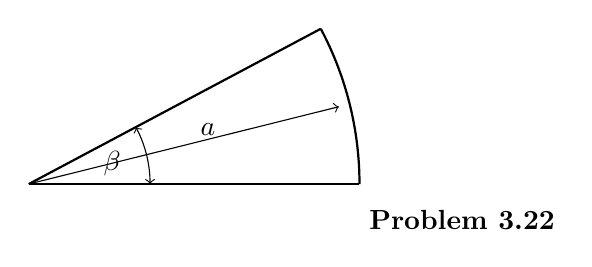
\begin{tikzpicture}[scale=1.4]
  % circular sector 0<=phi<=beta, rho<=a
  \draw[thick] (0,0) -- (3.0,0);
  \draw[thick] (0,0) -- (28:3.0);
  \draw[thick] (3.0,0) arc (0:28:3.0);
  % radial arrow a along the bisector
  \draw[->] (0,0) -- (14:2.9);
  \node at (17:1.7) {$a$};
  % angle beta at apex
  \draw[<->] (1.1,0) arc (0:28:1.1);
  \node at (14:0.78) {$\beta$};
  \node[below right] at (3.0,-0.15) {\textbf{Problem 3.22}};
\end{tikzpicture}
\end{center}

Using separation of variables in polar coordinates, show that the Green function can be written as
\[
G(\rho,\phi;\rho',\phi')=\sum_{m=1}^{\infty}\frac{4}{m}\,\rho_{<}^{m\pi/\beta}\left(\frac{1}{\rho_{>}^{m\pi/\beta}}-\frac{\rho_{>}^{m\pi/\beta}}{a^{2m\pi/\beta}}\right)\sin\!\left(\frac{m\pi\phi}{\beta}\right)\sin\!\left(\frac{m\pi\phi'}{\beta}\right)
\]
Problem 2.25 may be of use.
\solution

Use the two-dimensional convention
$\nabla^2G=-4\pi\delta(\rho-\rho')\delta(\phi-\phi')/\rho$.
On the interval $0<\phi<\beta$ the normalized delta expansion is
\[
\delta(\phi-\phi')=\frac2\beta\sum_{m=1}^\infty
\sin(\nu_m\phi)\sin(\nu_m\phi'),\qquad\nu_m=m\pi/\beta.
\]
Write $G=\sum_m g_m(\rho,\rho')\sin(\nu_m\phi)\sin(\nu_m\phi')$.
The radial equation is
\[
\left[\frac1\rho\frac d{d\rho}\rho\frac d{d\rho}
-\frac{\nu_m^2}{\rho^2}\right]g_m
=-\frac{8\pi}{\beta}\frac{\delta(\rho-\rho')}{\rho}.
\]
Its homogeneous solutions are $\rho^{\nu_m}$ and $\rho^{-\nu_m}$.
Regularity at the apex and the zero value at $a$ require
\[
g_m=C_m\rho_<^{\nu_m}
(\rho_>^{-\nu_m}-\rho_>^{\nu_m}/a^{2\nu_m}).
\]
This is continuous at $\rho'$; its derivative jump is
$[\rho\partial_\rho g_m]_-^+=-2\nu_mC_m$.
Integrating the radial equation across the source then fixes
$C_m=4\pi/(\beta\nu_m)=4/m$, proving the required formula.
Both radial faces and the arc have zero potential, the apex solution
is regular, and interchange of source and observation coordinates
leaves the result invariant.

\Needspace{5\baselineskip}
\par\bigskip
\noindent\textbf{3.23}\quad A point charge $q$ is located at the point $(\rho',\phi',z')$ inside a grounded cylindrical box defined by the surfaces $z=0$, $z=L$, $\rho=a$. Show that the potential inside the box can be expressed in the following alternative forms:
\begin{align*}
\Phi(\mathbf{x},\mathbf{x}')&=\frac{q}{\pi\epsilon_{0}a}\sum_{m=-\infty}^{\infty}\sum_{n=1}^{\infty}\frac{e^{im(\phi-\phi')}J_{m}\!\left(\dfrac{x_{mn}\rho}{a}\right)\!J_{m}\!\left(\dfrac{x_{mn}\rho'}{a}\right)}{x_{mn}J_{m+1}^{2}(x_{mn})\sinh\!\left(\dfrac{x_{mn}L}{a}\right)}\\
&\qquad\qquad\times\sinh\!\left[\frac{x_{mn}}{a}z_{<}\right]\sinh\!\left[\frac{x_{mn}}{a}(L-z_{>})\right]\\[6pt]
\Phi(\mathbf{x},\mathbf{x}')&=\frac{q}{\pi\epsilon_{0}L}\sum_{m=-\infty}^{\infty}\sum_{n=1}^{\infty}e^{im(\phi-\phi')}\sin\!\left(\frac{n\pi z}{L}\right)\sin\!\left(\frac{n\pi z'}{L}\right)\frac{I_{m}\!\left(\dfrac{n\pi\rho_{<}}{L}\right)}{I_{m}\!\left(\dfrac{n\pi a}{L}\right)}\\
&\qquad\qquad\times\left[I_{m}\!\left(\frac{n\pi a}{L}\right)\!K_{m}\!\left(\frac{n\pi\rho_{>}}{L}\right)-K_{m}\!\left(\frac{n\pi a}{L}\right)\!I_{m}\!\left(\frac{n\pi\rho_{>}}{L}\right)\right]\\[6pt]
\Phi(\mathbf{x},\mathbf{x}')&=\frac{2q}{\pi\epsilon_{0}La^{2}}\sum_{m=-\infty}^{\infty}\sum_{k=1}^{\infty}\sum_{n=1}^{\infty}\frac{e^{im(\phi-\phi')}\sin\!\left(\dfrac{k\pi z}{L}\right)\sin\!\left(\dfrac{k\pi z'}{L}\right)\!J_{m}\!\left(\dfrac{x_{mn}\rho}{a}\right)\!J_{m}\!\left(\dfrac{x_{mn}\rho'}{a}\right)}{\left[\left(\dfrac{x_{mn}}{a}\right)^{2}+\left(\dfrac{k\pi}{L}\right)^{2}\right]\!J_{m+1}^{2}(x_{mn})}
\end{align*}
Discuss the relation of the last expansion (with its extra summation) to the other two.
\solution

Use $\Phi=qG_D/(4\pi\epsilon_0)$ and denote the positive zeros
of $J_m$ by $x_{mn}$ (for negative $m$, use the corresponding zeros
of $J_{|m|}$).  The radial norm and completeness relation are
\[
\int_0^a\rho J_m(x_{mn}\rho/a)J_m(x_{mn'}\rho/a)d\rho
=\frac{a^2}2J_{m+1}^2(x_{mn})\delta_{nn'},
\]
\[
\frac{\delta(\rho-\rho')}{\rho}
=\frac2{a^2}\sum_{n=1}^\infty
\frac{J_m(x_{mn}\rho/a)J_m(x_{mn}\rho'/a)}{J_{m+1}^2(x_{mn})}.
\]
The sign in $J_{-m}=(-1)^mJ_m$ cancels in the products and norms.

First use this radial basis and angular Fourier modes.  For
$\alpha=x_{mn}/a$, the axial inverse of $-\partial_z^2+\alpha^2$
is
\[
h_\alpha(z,z')=
\frac{\sinh(\alpha z_<)\sinh[\alpha(L-z_>)]}{\alpha\sinh(\alpha L)},
\qquad [\partial_zh_\alpha]_-^+=-1.
\]
The source normalization gives
\[
G_D=\frac4{a^2}\sum_{m,n}
\frac{e^{im(\phi-\phi')}J_m(x_{mn}\rho/a)J_m(x_{mn}\rho'/a)}
{J_{m+1}^2(x_{mn})}\,h_{x_{mn}/a}(z,z').
\]
Multiplying by $q/(4\pi\epsilon_0)$ and using $\alpha=x_{mn}/a$
is exactly the first displayed potential.

Alternatively expand in axial sine modes with $\kappa=n\pi/L$.
The radial function satisfying both regularity and the wall condition is
\[
R_m(\rho,\rho';\kappa)=I_m(\kappa\rho_<)
\left[K_m(\kappa\rho_>)-
\frac{K_m(\kappa a)}{I_m(\kappa a)}I_m(\kappa\rho_>)\right].
\]
Its derivative jump is $[\rho\partial_\rho R_m]_-^+=-1$, by
the $I_m,K_m$ Wronskian.  Therefore
\[
G_D=\frac4L\sum_{m,n}e^{im(\phi-\phi')}
\sin(\kappa z)\sin(\kappa z')R_m(\rho,\rho';\kappa),
\]
which, after rearranging the bracket, gives the second potential.

Finally expand in both sets of eigenfunctions.  Their full
Laplacian eigenvalue is $\alpha^2+\kappa^2$, so inversion gives
\[
G_D=\frac8{La^2}\sum_{m,k,n}
\frac{e^{im(\phi-\phi')}\sin(k\pi z/L)\sin(k\pi z'/L)
J_m(x_{mn}\rho/a)J_m(x_{mn}\rho'/a)}
{[(x_{mn}/a)^2+(k\pi/L)^2]J_{m+1}^2(x_{mn})}.
\]
This is the third expression with its correct factor after multiplying
by $q/(4\pi\epsilon_0)$.  The extra sum has simply left both
one-dimensional inversions in spectral form.  Explicitly,
\[
\frac2L\sum_{k=1}^\infty
\frac{\sin(k\pi z/L)\sin(k\pi z'/L)}{\alpha^2+(k\pi/L)^2}
=h_\alpha(z,z'),
\]
reduces the third expression to the first; the radial resolvent
\[
\frac2{a^2}\sum_n
\frac{J_m(x_{mn}\rho/a)J_m(x_{mn}\rho'/a)}
{[(x_{mn}/a)^2+\kappa^2]J_{m+1}^2(x_{mn})}
=R_m(\rho,\rho';\kappa)
\]
reduces it to the second.  All three have the same boundary values,
source jump, and reciprocity, so uniqueness also establishes their
equivalence.

\Needspace{5\baselineskip}
\par\bigskip
\noindent\textbf{3.24}\quad The walls of the conducting cylindrical box of Problem 3.23 are all at zero potential, except for a disc in the upper end, defined by $\rho=b<a$, at potential $V$.
\begin{enumerate}
\item[(a)] Using the various forms of the Green function obtained in Problem 3.23, find three expansions for the potential inside the cylinder.
\item[(b)] For each series, calculate numerically the ratio of the potential at $\rho=0$, $z=L/2$ to the potential of the disc, assuming $b=L/4=a/2$. Try to obtain at least two-significant-figure accuracy. Is one series less rapidly convergent than the others? Why?
\end{enumerate}
(\emph{Abramowitz and Stegun} have tables; \emph{Mathematica} has Bessel functions, as does the software of \emph{Press et al.})
\solution

\textbf{(a)} Only the upper disc contributes to the Dirichlet
boundary formula,
\[
\Phi=-\frac V{4\pi}\int_0^{2\pi}d\phi'\int_0^b\rho'd\rho'
\,\partial_{z'}G_D(\rho,\phi,z;\rho',\phi',L).
\]
The angular integral selects $m=0$.  Put $x_n=x_{0n}$,
$\alpha_n=x_n/a$, and $\kappa_k=k\pi/L$.
In the first form of Problem 3.23, the upper-end derivative of
$h_{\alpha_n}$ is $-\sinh(\alpha_nz)/\sinh(\alpha_nL)$.
Using $\int_0^b\rho'J_0(\alpha_n\rho')d\rho'=bJ_1(\alpha_nb)/\alpha_n$
gives the first expansion:
\[
\boxed{\frac\Phi V=\frac{2b}a\sum_{n=1}^\infty
\frac{J_1(x_nb/a)}{x_nJ_1^2(x_n)}J_0(x_n\rho/a)
\frac{\sinh(x_nz/a)}{\sinh(x_nL/a)}.}\tag{A}
\]
For the second Green function define
$c_k=K_0(\kappa_ka)/I_0(\kappa_ka)$ and
\[
H_k(\rho)=\int_0^b\rho'I_0(\kappa_k\rho_<)
[K_0(\kappa_k\rho_>)-c_kI_0(\kappa_k\rho_>)]d\rho'.
\]
The primitive integrals are
$\int\rho I_0(\kappa\rho)d\rho=\rho I_1(\kappa\rho)/\kappa$
and $\int\rho K_0(\kappa\rho)d\rho=-\rho K_1(\kappa\rho)/\kappa$.
Splitting at $\rho'=\rho$ and using
$I_0(x)K_1(x)+I_1(x)K_0(x)=1/x$ yields
\[
H_k(\rho)=\begin{cases}
\kappa_k^{-2}-\dfrac b{\kappa_k}I_0(\kappa_k\rho)
[K_1(\kappa_kb)+c_kI_1(\kappa_kb)],&\rho\leq b,\\[3pt]
\dfrac b{\kappa_k}I_1(\kappa_kb)
[K_0(\kappa_k\rho)-c_kI_0(\kappa_k\rho)],&b\leq\rho<a.
\end{cases}
\]
The second expansion is therefore
\[
\boxed{\frac\Phi V=\frac2L\sum_{k=1}^\infty
(-1)^{k+1}\kappa_k\sin(\kappa_kz)H_k(\rho).}\tag{B}
\]
The third Green function gives directly
\[
\boxed{\frac\Phi V=\frac{4b}{La}\sum_{n=1}^\infty\sum_{k=1}^\infty
\frac{(-1)^{k+1}\kappa_k\sin(\kappa_kz)
J_0(x_n\rho/a)J_1(x_nb/a)}
{x_nJ_1^2(x_n)(\alpha_n^2+\kappa_k^2)}.}\tag{C}
\]
As a boundary limit these are interpreted in the usual Fourier/Abel
sense at jumps.  For strictly interior points they give the same
harmonic solution.

\textbf{(b)} Choose units $a=1$, so $b=1/2$, $L=2$, $z=1$.
The factor in (A) is $\sinh x_n/\sinh2x_n=1/(2\cosh x_n)$.
Its partial sums are
\[
\begin{array}{c|rrrr}
N&1&2&5&10\\\hline
\Phi_A/V&0.06893268&0.07158219&0.07152937&0.07152937289
\end{array}
\]
For (B) the raw sums and an accelerated evaluation are
\[
\begin{array}{c|rrrr}
K&11&51&101&501\\\hline
\Phi_B/V&0.04518810&0.06541029&0.07464976&0.07216345
\end{array}
\]
The slow part can be summed exactly:
$(2/\pi)\sum_{k\geq1}(-1)^{k+1}\sin(k\pi z/L)/k=z/L$.
Subtracting this $1/k$ tail from (B), summing the remaining Bessel
terms, and adding $z/L$ gives $0.07152937289$ (51 terms suffice).

For (C), rectangular sums over $(N,K)=(20,51),(100,501),(200,2001)$
give respectively $0.06595877$, $0.07212779$, and $0.07168131$.
An independent acceleration is Euler's transformation of the
alternating odd-$k$ sum at $z=L/2$.  If it is
$\sum_{j\geq0}(-1)^ju_j$, use
$\sum_{p\geq0}\Delta^pu_0/2^{p+1}$ with
$\Delta u_j=u_j-u_{j+1}$.  Taking $N=20$ radial modes and 32 odd
axial terms gives $0.071529372893$; increasing to $(40,64)$ gives
$0.071529372888$.  Thus every representation yields
\[
\boxed{\Phi(0,L/2)/V=0.07152937289\ldots\simeq0.072.}
\]
Series (A) has exponential suppression across the distance from the
upper boundary.  The unaccelerated axial sine series (B) and (C)
retain a $1/k$ tail because their basis functions vanish at the end
where the imposed boundary value jumps to a nonzero value.  The
extra unsummed spectrum in (C) adds work without accelerating that
tail.  The supplementary code reproduces all three calculations.

\Needspace{5\baselineskip}
\par\bigskip
\noindent\textbf{3.25}\quad Consider the surface-charge densities for the problem of Section 3.13 of the conducting plane with a circular hole of radius $a$.
\begin{enumerate}
\item[(a)] Show that the surface-charge densities on the top and bottom of the plane for $\rho\geq a$ are
\begin{align*}
\sigma_{+}(\rho)&=-\epsilon_{0}E_{0}+\Delta\sigma(\rho)\\
\sigma_{-}(\rho)&=\epsilon_{0}E_{1}+\Delta\sigma(\rho)
\end{align*}
where
\[
\Delta\sigma(\rho)=-\epsilon_{0}\frac{(E_{0}-E_{1})}{\pi}\left[\frac{a}{\sqrt{\rho^{2}-a^{2}}}-\sin^{-1}\!\left(\frac{a}{\rho}\right)\right]
\]
How does $\Delta\sigma(\rho)$ behave for large $\rho$? Is $\Delta\sigma(\rho)$, defined in terms of $\Phi^{(1)}$, zero for $\rho<a$? Explain.
\item[(b)] Show by direct integration that
\[
\lim_{R\to\infty}\left[2\pi\int_{a}^{R}d\rho\;\rho(\sigma_{+}+\sigma_{-})+2\pi\epsilon_{0}\int_{0}^{R}d\rho\;\rho(E_{0}-E_{1})\right]=0
\]
Interpret.
\end{enumerate}
\solution

Put $\Delta E=E_0-E_1$.  Section 3.13 gives
$\Phi=E_0z+\Phi^{(1)}$ above and $\Phi=E_1z+\Phi^{(1)}$ below,
where the even correction has the transform
\[
\Phi^{(1)}=\frac{\Delta E}{\pi}\int_0^\infty
\left[\frac{\sin(ka)}{k^2}-\frac{a\cos(ka)}k\right]
e^{-k|z|}J_0(k\rho)dk.
\]
\textbf{(a)} On the upper conducting face
$\sigma_+=-\epsilon_0\partial_z\Phi|_{0^+}$, so its correction is
\[
\Delta\sigma=\frac{\epsilon_0\Delta E}{\pi}
\left[\int_0^\infty\frac{\sin(ka)}kJ_0(k\rho)dk
-a\int_0^\infty\cos(ka)J_0(k\rho)dk\right].
\]
For $\rho>a$, take the real part of
$\int_0^\infty e^{-(s-ia)k}J_0(k\rho)dk
=[(s-ia)^2+\rho^2]^{-1/2}$ as $s\downarrow0$ to get
$(\rho^2-a^2)^{-1/2}$.  Integration with respect to $a$ from zero
gives the first integral $\sin^{-1}(a/\rho)$.
Hence the stated expression for $\Delta\sigma$ follows.
Evenness of $\Phi^{(1)}$ makes the correction on the bottom face
the same, whereas the background contribution has the opposite
normal sign.  Thus $\sigma_+=-\epsilon_0E_0+\Delta\sigma$ and
$\sigma_-=\epsilon_0E_1+\Delta\sigma$.
At large $\rho$, set $t=a/\rho$ and expand:
\[
\frac{t}{\sqrt{1-t^2}}-\sin^{-1}t
=\frac{t^3}3+\frac{3t^5}{10}+O(t^7),\quad
\Delta\sigma=-\frac{\epsilon_0\Delta E\,a^3}{3\pi\rho^3}
+O(\rho^{-5}).
\]
Inside the hole the second transform is zero while the first is
$\pi/2$.  Therefore the correction \emph{defined from}
$\Phi^{(1)}$ is $\Delta\sigma=\epsilon_0\Delta E/2$ per face,
not zero.  It is a fictitious correction to the intact-plane
background: the combined correction $2\Delta\sigma$ cancels its
background sheet charge $-\epsilon_0\Delta E$ in the hole.
There is no physical surface charge where the material is absent.

\textbf{(b)} A direct primitive gives
\begin{align*}
I(R)&=\int_a^R\rho\left[
\frac a{\sqrt{\rho^2-a^2}}-\sin^{-1}\frac a\rho\right]d\rho\\
&=\frac a2\sqrt{R^2-a^2}-\frac{R^2}2\sin^{-1}(a/R)
+\frac{\pi a^2}4\longrightarrow\frac{\pi a^2}4.
\end{align*}
The quantity in the question equals
\[
\pi\epsilon_0\Delta E\,a^2-4\epsilon_0\Delta E I(R)
=2\epsilon_0\Delta E\left[R^2\sin^{-1}(a/R)
-a\sqrt{R^2-a^2}\right]
=\frac{4\epsilon_0\Delta E\,a^3}{3R}+O(R^{-3}),
\]
and therefore tends to zero.  The missing intact-plane charge in
the hole is exactly compensated by the redistribution on the
remaining conductor.  Equivalently, the total charge associated
with $\Phi^{(1)}$ is zero, consistent with its absence of a monopole
far field.

\Needspace{5\baselineskip}
\par\bigskip
\noindent\textbf{3.26}\quad Consider the Green function appropriate for Neumann boundary conditions for the volume $V$ between the concentric spherical surfaces defined by $r=a$ and $r=b$, $a<b$. To be able to use (1.46) for the potential, impose the simple constraint (1.45). Use an expansion in spherical harmonics of the form,
\[
G(\mathbf{x},\mathbf{x}')=\sum_{l=0}^{\infty}g_{l}(r,r')P_{l}(\cos\gamma)
\]
where $g_{l}(r,r')=r_{<}^{l}/r_{>}^{l+1}+f_{l}(r,r')$.
\begin{enumerate}
\item[(a)] Show that for $l>0$, the radial Green function has the symmetric form
\begin{align*}
g_{l}(r,r')=\frac{r_{<}^{l}}{r_{>}^{l+1}}&+\\
\frac{1}{(b^{2l+1}-a^{2l+1})}&\left[\frac{l+1}{l}(rr')^{l}+\frac{l}{l+1}\frac{(ab)^{2l+1}}{(rr')^{l+1}}+a^{2l+1}\!\left(\frac{r^{l}}{r'^{\,l+1}}+\frac{r'^{\,l}}{r^{l+1}}\right)\right]
\end{align*}
\item[(b)] Show that for $l=0$
\[
g_{0}(r,r')=\frac{1}{r_{>}}-\left(\frac{a^{2}}{a^{2}+b^{2}}\right)\frac{1}{r'}+f(r)
\]
where $f(r)$ is arbitrary. Show explicitly in (1.46) that answers for the potential $\Phi(\mathbf{x})$ are independent of $f(r)$.

[The arbitrariness in the Neumann Green function can be removed by symmetrizing $g_{0}$ in $r$ and $r'$ with a suitable choice of $f(r)$.]
\end{enumerate}
\solution

The Neumann convention of Eqs.~(1.45)--(1.46) is
\[
\nabla'^2G_N=-4\pi\delta^3(\mathbf r-\mathbf r'),\qquad
\partial_{n'}G_N=-\frac{4\pi}{S}
=-\frac1{a^2+b^2},\quad S=4\pi(a^2+b^2).
\]
The inner outward normal is $-\hat{\mathbf r}'$ and the outer
normal is $+\hat{\mathbf r}'$.

\textbf{(a)} For $l>0$ the boundary derivative must vanish.  Write
\[
f_l=A_l(r)r'^l+B_l(r)r'^{-l-1}.
\]
At $r'=a<r$, differentiating the Coulomb term and $f_l$ gives
\[
A_l-\frac{l+1}{l}\frac{B_l}{a^{2l+1}}=-r^{-l-1}.
\]
At $r'=b>r$ the analogous condition is
\[
\frac l{l+1}A_lb^{2l+1}-B_l=r^l.
\]
Eliminating $A_l,B_l$, with $D_l=b^{2l+1}-a^{2l+1}$, yields
\[
A_l=\frac{(l+1)r^l/l+a^{2l+1}r^{-l-1}}{D_l},\qquad
B_l=\frac{a^{2l+1}r^l+[l/(l+1)](ab)^{2l+1}r^{-l-1}}{D_l}.
\]
Insertion into $f_l$ gives
\[
\boxed{g_l=\frac{r_<^l}{r_>^{l+1}}+\frac1{D_l}
\left[\frac{l+1}{l}(rr')^l+
\frac l{l+1}\frac{(ab)^{2l+1}}{(rr')^{l+1}}
+a^{2l+1}\left(\frac{r^l}{r'^{l+1}}+
\frac{r'^l}{r^{l+1}}\right)\right].}
\]
It is explicitly symmetric and has the same source derivative jump
as the Coulomb radial term; the added terms are harmonic in the
source coordinate.

\textbf{(b)} Put $c=a^2/(a^2+b^2)$.  For $l=0$ the proposed form
\[
g_0=\frac1{r_>}-\frac c{r'}+f(r)
\]
is harmonic in $r'$ away from the source.  Its inner radial derivative
is $c/a^2=1/(a^2+b^2)$ and its outer derivative is
$(-1+c)/b^2=-1/(a^2+b^2)$, exactly the required normal derivatives.
The function $f(r)$ is arbitrary because the defining differential
equation and boundary constraint act on the primed argument.
Choosing $f(r)=-c/r+C$ makes $g_0$ symmetric.

To verify that this freedom is immaterial, write the Neumann
representation with $\varrho$ denoting the volume charge density:
\[
\Phi(\mathbf r)-\langle\Phi\rangle_S
=\frac1{4\pi\epsilon_0}\int_V\varrho(\mathbf r')G_N\,d^3r'
+\frac1{4\pi}\oint_SG_N\partial_{n'}\Phi\,dS',
\quad\langle\Phi\rangle_S=\frac1S\oint_S\Phi\,dS.
\]
Changing $f$ by $\delta f(r)$ changes its right side by
\[
\frac{\delta f(r)}{4\pi}
\left[\frac{Q_V}{\epsilon_0}+\oint_S\partial_n\Phi\,dS\right]=0,
\]
because Gauss's law/Poisson's equation gives
$\oint_S\partial_n\Phi\,dS=-Q_V/\epsilon_0$.
This is also the compatibility condition for the prescribed Neumann
data.  Only the arbitrary additive constant in $\Phi$ remains.

\Needspace{5\baselineskip}
\par\bigskip
\noindent\textbf{3.27}\quad Apply the Neumann Green function of Problem 3.26 to the situation in which the normal electric field is $E_{r}=-E_{0}\cos\theta$ at the outer surface ($r=b$) and is $E_{r}=0$ on the inner surface ($r=a$).
\begin{enumerate}
\item[(a)] Show that the electrostatic potential inside the volume $V$ is
\[
\Phi(\mathbf{x})=E_{0}\,\frac{r\cos\theta}{1-p^{3}}\left(1+\frac{a^{3}}{2r^{3}}\right)
\]
where $p=a/b$. Find the components of the electric field,
\[
E_{r}(r,\theta)=-E_{0}\,\frac{\cos\theta}{1-p^{3}}\left(1-\frac{a^{3}}{r^{3}}\right),\qquad
E_{\theta}(r,\theta)=E_{0}\,\frac{\sin\theta}{1-p^{3}}\left(1+\frac{a^{3}}{2r^{3}}\right)
\]
\item[(b)] Calculate the Cartesian or cylindrical components of the field, $E_{z}$ and $E_{\rho}$, and make a sketch or computer plot of the lines of electric force for a typical case of $p=0.5$.
\end{enumerate}
\solution

\textbf{(a)} There is no volume charge.  On $r=b$,
$\partial_n\Phi=\partial_r\Phi=-E_r=E_0\cos\theta$;
on $r=a$ the derivative is zero.  Choose the additive constant so
that the surface average of $\Phi$ is zero.  The Neumann formula is
then
\[
\Phi=\frac{E_0b^2}{4\pi}\int G_N(\mathbf r,b\hat{\mathbf r}')
\cos\theta'\,d\Omega'.
\]
The angular addition theorem gives
$\int P_l(\cos\gamma)\cos\theta'\,d\Omega'
=(4\pi/3)\delta_{l1}\cos\theta$.  From Problem 3.26,
\[
g_1(r,b)=\frac{3}{b^2(1-a^3/b^3)}
\left(r+\frac{a^3}{2r^2}\right).
\]
Thus, with $p=a/b$,
\[
\boxed{\Phi=\frac{E_0}{1-p^3}\left(r+\frac{a^3}{2r^2}\right)
\cos\theta.}
\]
Differentiating, $E_r=-\partial_r\Phi$ and
$E_\theta=-r^{-1}\partial_\theta\Phi$, gives exactly
\[
E_r=-\frac{E_0}{1-p^3}(1-a^3/r^3)\cos\theta,\qquad
E_\theta=\frac{E_0}{1-p^3}(1+a^3/(2r^3))\sin\theta.
\]
In particular $E_r(a)=0$ and $E_r(b)=-E_0\cos\theta$, checking
both Neumann conditions.

\textbf{(b)} Resolve the unit vectors along and perpendicular to
$z$: $E_z=E_r\cos\theta-E_\theta\sin\theta$,
$E_\rho=E_r\sin\theta+E_\theta\cos\theta$.  If
$K=E_0/(1-p^3)$, this gives
\[
\boxed{E_z=-K\left[1-\frac{a^3}{2r^3}(3\cos^2\theta-1)\right],
\qquad E_\rho=\frac{3Ka^3}{2r^3}\sin\theta\cos\theta.}
\]
Equivalently $E_\rho=3Ka^3\rho z/(2r^5)$ and
$E_z=-K[1-a^3(2z^2-\rho^2)/(2r^5)]$.
A useful axisymmetric flux function is
\[
\Psi=-\frac K2\left(r^2-\frac{a^3}{r}\right)\sin^2\theta,
\quad
E_r=\frac{\partial_\theta\Psi}{r^2\sin\theta},\quad
E_\theta=-\frac{\partial_r\Psi}{r\sin\theta}.
\]
Hence field lines have constant
\[
\boxed{\rho^2\left[1-\frac{a^3}{(\rho^2+z^2)^{3/2}}\right].}
\]
This exact first integral was used to generate the following
meridional section for $p=0.5$ and $E_0>0$.  Arrows run from the
upper outer hemisphere to the lower one; the inner sphere is a
zero-normal-flux surface.  Rotation about $z$ gives the full field.
\begin{center}
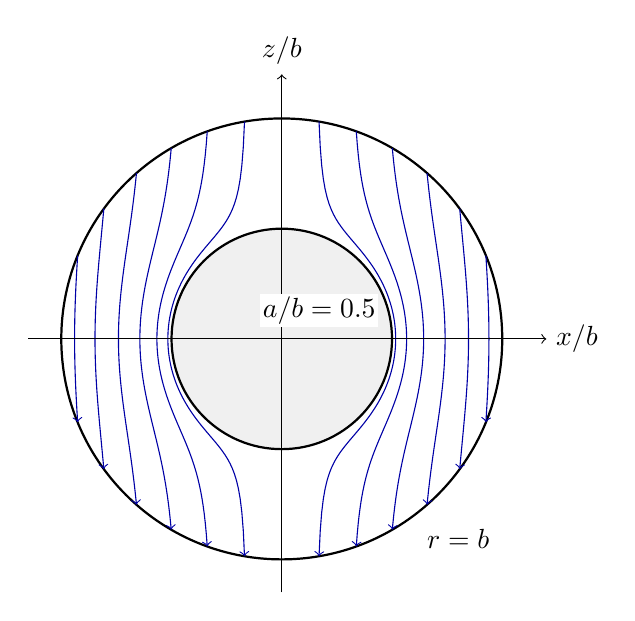
\begin{tikzpicture}[scale=2.8]
\draw[thick] (0,0) circle (1);
\filldraw[fill=gray!12,draw=black,thick] (0,0) circle (.5);
\draw[blue!65!black,thin,->] plot coordinates {(-0.1690309,0.9856108) (-0.1744767,0.8702578) (-0.1809944,0.7875959) (-0.1884470,0.7261819) (-0.1966835,0.6790696) (-0.2055576,0.6418404) (-0.2149375,0.6115847) (-0.2247093,0.5863337) (-0.2347763,0.5647238) (-0.2450574,0.5457918) (-0.2554847,0.5288444) (-0.2660007,0.5133747) (-0.2765572,0.4990062) (-0.2871127,0.4854560) (-0.2976314,0.4725088) (-0.3080824,0.4599989) (-0.3184382,0.4477980) (-0.3286747,0.4358056) (-0.3387702,0.4239429) (-0.3487052,0.4121477) (-0.3584619,0.4003707) (-0.3680241,0.3885729) (-0.3773769,0.3767237) (-0.3865064,0.3647988) (-0.3953999,0.3527794) (-0.4040455,0.3406510) (-0.4124320,0.3284029) (-0.4205491,0.3160273) (-0.4283870,0.3035187) (-0.4359366,0.2908740) (-0.4431892,0.2780919) (-0.4501367,0.2651724) (-0.4567717,0.2521169) (-0.4630870,0.2389280) (-0.4690760,0.2256092) (-0.4747324,0.2121648) (-0.4800504,0.1985999) (-0.4850247,0.1849202) (-0.4896503,0.1711320) (-0.4939225,0.1572421) (-0.4978372,0.1432577) (-0.5013905,0.1291862) (-0.5045790,0.1150355) (-0.5073996,0.1008139) (-0.5098496,0.0865296) (-0.5119267,0.0721913) (-0.5136288,0.0578077) (-0.5149543,0.0433877) (-0.5159020,0.0289404) (-0.5164710,0.0144748) (-0.5166607,-0.0000000) (-0.5164710,-0.0144748) (-0.5159020,-0.0289404) (-0.5149543,-0.0433877) (-0.5136288,-0.0578077) (-0.5119267,-0.0721913) (-0.5098496,-0.0865296) (-0.5073996,-0.1008139) (-0.5045790,-0.1150355) (-0.5013905,-0.1291862) (-0.4978372,-0.1432577) (-0.4939225,-0.1572421) (-0.4896503,-0.1711320) (-0.4850247,-0.1849202) (-0.4800504,-0.1985999) (-0.4747324,-0.2121648) (-0.4690760,-0.2256092) (-0.4630870,-0.2389280) (-0.4567717,-0.2521169) (-0.4501367,-0.2651724) (-0.4431892,-0.2780919) (-0.4359366,-0.2908740) (-0.4283870,-0.3035187) (-0.4205491,-0.3160273) (-0.4124320,-0.3284029) (-0.4040455,-0.3406510) (-0.3953999,-0.3527794) (-0.3865064,-0.3647988) (-0.3773769,-0.3767237) (-0.3680241,-0.3885729) (-0.3584619,-0.4003707) (-0.3487052,-0.4121477) (-0.3387702,-0.4239429) (-0.3286747,-0.4358056) (-0.3184382,-0.4477980) (-0.3080824,-0.4599989) (-0.2976314,-0.4725088) (-0.2871127,-0.4854560) (-0.2765572,-0.4990062) (-0.2660007,-0.5133747) (-0.2554847,-0.5288444) (-0.2450574,-0.5457918) (-0.2347763,-0.5647238) (-0.2247093,-0.5863337) (-0.2149375,-0.6115847) (-0.2055576,-0.6418404) (-0.1966835,-0.6790696) (-0.1884470,-0.7261819) (-0.1809944,-0.7875959) (-0.1744767,-0.8702578) (-0.1690309,-0.9856108)};
\draw[blue!65!black,thin,->] plot coordinates {(0.1690309,0.9856108) (0.1744767,0.8702578) (0.1809944,0.7875959) (0.1884470,0.7261819) (0.1966835,0.6790696) (0.2055576,0.6418404) (0.2149375,0.6115847) (0.2247093,0.5863337) (0.2347763,0.5647238) (0.2450574,0.5457918) (0.2554847,0.5288444) (0.2660007,0.5133747) (0.2765572,0.4990062) (0.2871127,0.4854560) (0.2976314,0.4725088) (0.3080824,0.4599989) (0.3184382,0.4477980) (0.3286747,0.4358056) (0.3387702,0.4239429) (0.3487052,0.4121477) (0.3584619,0.4003707) (0.3680241,0.3885729) (0.3773769,0.3767237) (0.3865064,0.3647988) (0.3953999,0.3527794) (0.4040455,0.3406510) (0.4124320,0.3284029) (0.4205491,0.3160273) (0.4283870,0.3035187) (0.4359366,0.2908740) (0.4431892,0.2780919) (0.4501367,0.2651724) (0.4567717,0.2521169) (0.4630870,0.2389280) (0.4690760,0.2256092) (0.4747324,0.2121648) (0.4800504,0.1985999) (0.4850247,0.1849202) (0.4896503,0.1711320) (0.4939225,0.1572421) (0.4978372,0.1432577) (0.5013905,0.1291862) (0.5045790,0.1150355) (0.5073996,0.1008139) (0.5098496,0.0865296) (0.5119267,0.0721913) (0.5136288,0.0578077) (0.5149543,0.0433877) (0.5159020,0.0289404) (0.5164710,0.0144748) (0.5166607,-0.0000000) (0.5164710,-0.0144748) (0.5159020,-0.0289404) (0.5149543,-0.0433877) (0.5136288,-0.0578077) (0.5119267,-0.0721913) (0.5098496,-0.0865296) (0.5073996,-0.1008139) (0.5045790,-0.1150355) (0.5013905,-0.1291862) (0.4978372,-0.1432577) (0.4939225,-0.1572421) (0.4896503,-0.1711320) (0.4850247,-0.1849202) (0.4800504,-0.1985999) (0.4747324,-0.2121648) (0.4690760,-0.2256092) (0.4630870,-0.2389280) (0.4567717,-0.2521169) (0.4501367,-0.2651724) (0.4431892,-0.2780919) (0.4359366,-0.2908740) (0.4283870,-0.3035187) (0.4205491,-0.3160273) (0.4124320,-0.3284029) (0.4040455,-0.3406510) (0.3953999,-0.3527794) (0.3865064,-0.3647988) (0.3773769,-0.3767237) (0.3680241,-0.3885729) (0.3584619,-0.4003707) (0.3487052,-0.4121477) (0.3387702,-0.4239429) (0.3286747,-0.4358056) (0.3184382,-0.4477980) (0.3080824,-0.4599989) (0.2976314,-0.4725088) (0.2871127,-0.4854560) (0.2765572,-0.4990062) (0.2660007,-0.5133747) (0.2554847,-0.5288444) (0.2450574,-0.5457918) (0.2347763,-0.5647238) (0.2247093,-0.5863337) (0.2149375,-0.6115847) (0.2055576,-0.6418404) (0.1966835,-0.6790696) (0.1884470,-0.7261819) (0.1809944,-0.7875959) (0.1744767,-0.8702578) (0.1690309,-0.9856108)};
\draw[blue!65!black,thin,->] plot coordinates {(-0.3380617,0.9411239) (-0.3423211,0.8842199) (-0.3469395,0.8347631) (-0.3518912,0.7913529) (-0.3571474,0.7528926) (-0.3626779,0.7185116) (-0.3684516,0.6875118) (-0.3744373,0.6593274) (-0.3806044,0.6334968) (-0.3869230,0.6096405) (-0.3933647,0.5874445) (-0.3999021,0.5666478) (-0.4065096,0.5470323) (-0.4131628,0.5284149) (-0.4198391,0.5106414) (-0.4265171,0.4935815) (-0.4331768,0.4771247) (-0.4397998,0.4611768) (-0.4463687,0.4456580) (-0.4528672,0.4304995) (-0.4592804,0.4156430) (-0.4655941,0.4010383) (-0.4717952,0.3866422) (-0.4778714,0.3724179) (-0.4838113,0.3583337) (-0.4896041,0.3443624) (-0.4952398,0.3304808) (-0.5007091,0.3166690) (-0.5060032,0.3029101) (-0.5111139,0.2891896) (-0.5160336,0.2754954) (-0.5207552,0.2618174) (-0.5252718,0.2481471) (-0.5295775,0.2344774) (-0.5336662,0.2208028) (-0.5375328,0.2071187) (-0.5411723,0.1934218) (-0.5445799,0.1797094) (-0.5477516,0.1659799) (-0.5506834,0.1522323) (-0.5533718,0.1384660) (-0.5558136,0.1246813) (-0.5580059,0.1108787) (-0.5599463,0.0970594) (-0.5616324,0.0832246) (-0.5630623,0.0693760) (-0.5642345,0.0555155) (-0.5651476,0.0416453) (-0.5658005,0.0277678) (-0.5661925,0.0138851) (-0.5663232,0.0000000) (-0.5661925,-0.0138851) (-0.5658005,-0.0277678) (-0.5651476,-0.0416453) (-0.5642345,-0.0555155) (-0.5630623,-0.0693760) (-0.5616324,-0.0832246) (-0.5599463,-0.0970594) (-0.5580059,-0.1108787) (-0.5558136,-0.1246813) (-0.5533718,-0.1384660) (-0.5506834,-0.1522323) (-0.5477516,-0.1659799) (-0.5445799,-0.1797094) (-0.5411723,-0.1934218) (-0.5375328,-0.2071187) (-0.5336662,-0.2208028) (-0.5295775,-0.2344774) (-0.5252718,-0.2481471) (-0.5207552,-0.2618174) (-0.5160336,-0.2754954) (-0.5111139,-0.2891896) (-0.5060032,-0.3029101) (-0.5007091,-0.3166690) (-0.4952398,-0.3304808) (-0.4896041,-0.3443624) (-0.4838113,-0.3583337) (-0.4778714,-0.3724179) (-0.4717952,-0.3866422) (-0.4655941,-0.4010383) (-0.4592804,-0.4156430) (-0.4528672,-0.4304995) (-0.4463687,-0.4456580) (-0.4397998,-0.4611768) (-0.4331768,-0.4771247) (-0.4265171,-0.4935815) (-0.4198391,-0.5106414) (-0.4131628,-0.5284149) (-0.4065096,-0.5470323) (-0.3999021,-0.5666478) (-0.3933647,-0.5874445) (-0.3869230,-0.6096405) (-0.3806044,-0.6334968) (-0.3744373,-0.6593274) (-0.3684516,-0.6875118) (-0.3626779,-0.7185116) (-0.3571474,-0.7528926) (-0.3518912,-0.7913529) (-0.3469395,-0.8347631) (-0.3423211,-0.8842199) (-0.3380617,-0.9411239)};
\draw[blue!65!black,thin,->] plot coordinates {(0.3380617,0.9411239) (0.3423211,0.8842199) (0.3469395,0.8347631) (0.3518912,0.7913529) (0.3571474,0.7528926) (0.3626779,0.7185116) (0.3684516,0.6875118) (0.3744373,0.6593274) (0.3806044,0.6334968) (0.3869230,0.6096405) (0.3933647,0.5874445) (0.3999021,0.5666478) (0.4065096,0.5470323) (0.4131628,0.5284149) (0.4198391,0.5106414) (0.4265171,0.4935815) (0.4331768,0.4771247) (0.4397998,0.4611768) (0.4463687,0.4456580) (0.4528672,0.4304995) (0.4592804,0.4156430) (0.4655941,0.4010383) (0.4717952,0.3866422) (0.4778714,0.3724179) (0.4838113,0.3583337) (0.4896041,0.3443624) (0.4952398,0.3304808) (0.5007091,0.3166690) (0.5060032,0.3029101) (0.5111139,0.2891896) (0.5160336,0.2754954) (0.5207552,0.2618174) (0.5252718,0.2481471) (0.5295775,0.2344774) (0.5336662,0.2208028) (0.5375328,0.2071187) (0.5411723,0.1934218) (0.5445799,0.1797094) (0.5477516,0.1659799) (0.5506834,0.1522323) (0.5533718,0.1384660) (0.5558136,0.1246813) (0.5580059,0.1108787) (0.5599463,0.0970594) (0.5616324,0.0832246) (0.5630623,0.0693760) (0.5642345,0.0555155) (0.5651476,0.0416453) (0.5658005,0.0277678) (0.5661925,0.0138851) (0.5663232,0.0000000) (0.5661925,-0.0138851) (0.5658005,-0.0277678) (0.5651476,-0.0416453) (0.5642345,-0.0555155) (0.5630623,-0.0693760) (0.5616324,-0.0832246) (0.5599463,-0.0970594) (0.5580059,-0.1108787) (0.5558136,-0.1246813) (0.5533718,-0.1384660) (0.5506834,-0.1522323) (0.5477516,-0.1659799) (0.5445799,-0.1797094) (0.5411723,-0.1934218) (0.5375328,-0.2071187) (0.5336662,-0.2208028) (0.5295775,-0.2344774) (0.5252718,-0.2481471) (0.5207552,-0.2618174) (0.5160336,-0.2754954) (0.5111139,-0.2891896) (0.5060032,-0.3029101) (0.5007091,-0.3166690) (0.4952398,-0.3304808) (0.4896041,-0.3443624) (0.4838113,-0.3583337) (0.4778714,-0.3724179) (0.4717952,-0.3866422) (0.4655941,-0.4010383) (0.4592804,-0.4156430) (0.4528672,-0.4304995) (0.4463687,-0.4456580) (0.4397998,-0.4611768) (0.4331768,-0.4771247) (0.4265171,-0.4935815) (0.4198391,-0.5106414) (0.4131628,-0.5284149) (0.4065096,-0.5470323) (0.3999021,-0.5666478) (0.3933647,-0.5874445) (0.3869230,-0.6096405) (0.3806044,-0.6334968) (0.3744373,-0.6593274) (0.3684516,-0.6875118) (0.3626779,-0.7185116) (0.3571474,-0.7528926) (0.3518912,-0.7913529) (0.3469395,-0.8347631) (0.3423211,-0.8842199) (0.3380617,-0.9411239)};
\draw[blue!65!black,thin,->] plot coordinates {(-0.5014265,0.8652002) (-0.5046849,0.8303045) (-0.5080681,0.7977946) (-0.5115664,0.7673876) (-0.5151695,0.7388389) (-0.5188668,0.7119359) (-0.5226476,0.6864932) (-0.5265011,0.6623485) (-0.5304165,0.6393592) (-0.5343829,0.6173999) (-0.5383898,0.5963595) (-0.5424267,0.5761398) (-0.5464832,0.5566538) (-0.5505493,0.5378240) (-0.5546153,0.5195814) (-0.5586716,0.5018644) (-0.5627091,0.4846181) (-0.5667190,0.4677934) (-0.5706927,0.4513462) (-0.5746219,0.4352371) (-0.5784989,0.4194307) (-0.5823160,0.4038952) (-0.5860660,0.3886022) (-0.5897421,0.3735259) (-0.5933376,0.3586434) (-0.5968463,0.3439340) (-0.6002623,0.3293789) (-0.6035797,0.3149615) (-0.6067933,0.3006666) (-0.6098979,0.2864807) (-0.6128888,0.2723917) (-0.6157614,0.2583886) (-0.6185114,0.2444616) (-0.6211347,0.2306018) (-0.6236276,0.2168014) (-0.6259867,0.2030533) (-0.6282085,0.1893511) (-0.6302900,0.1756890) (-0.6322284,0.1620621) (-0.6340212,0.1484658) (-0.6356658,0.1348960) (-0.6371603,0.1213490) (-0.6385026,0.1078215) (-0.6396910,0.0943105) (-0.6407240,0.0808135) (-0.6416003,0.0673280) (-0.6423188,0.0538517) (-0.6428785,0.0403827) (-0.6432789,0.0269189) (-0.6435192,0.0134586) (-0.6435994,0.0000000) (-0.6435192,-0.0134586) (-0.6432789,-0.0269189) (-0.6428785,-0.0403827) (-0.6423188,-0.0538517) (-0.6416003,-0.0673280) (-0.6407240,-0.0808135) (-0.6396910,-0.0943105) (-0.6385026,-0.1078215) (-0.6371603,-0.1213490) (-0.6356658,-0.1348960) (-0.6340212,-0.1484658) (-0.6322284,-0.1620621) (-0.6302900,-0.1756890) (-0.6282085,-0.1893511) (-0.6259867,-0.2030533) (-0.6236276,-0.2168014) (-0.6211347,-0.2306018) (-0.6185114,-0.2444616) (-0.6157614,-0.2583886) (-0.6128888,-0.2723917) (-0.6098979,-0.2864807) (-0.6067933,-0.3006666) (-0.6035797,-0.3149615) (-0.6002623,-0.3293789) (-0.5968463,-0.3439340) (-0.5933376,-0.3586434) (-0.5897421,-0.3735259) (-0.5860660,-0.3886022) (-0.5823160,-0.4038952) (-0.5784989,-0.4194307) (-0.5746219,-0.4352371) (-0.5706927,-0.4513462) (-0.5667190,-0.4677934) (-0.5627091,-0.4846181) (-0.5586716,-0.5018644) (-0.5546153,-0.5195814) (-0.5505493,-0.5378240) (-0.5464832,-0.5566538) (-0.5424267,-0.5761398) (-0.5383898,-0.5963595) (-0.5343829,-0.6173999) (-0.5304165,-0.6393592) (-0.5265011,-0.6623485) (-0.5226476,-0.6864932) (-0.5188668,-0.7119359) (-0.5151695,-0.7388389) (-0.5115664,-0.7673876) (-0.5080681,-0.7977946) (-0.5046849,-0.8303045) (-0.5014265,-0.8652002)};
\draw[blue!65!black,thin,->] plot coordinates {(0.5014265,0.8652002) (0.5046849,0.8303045) (0.5080681,0.7977946) (0.5115664,0.7673876) (0.5151695,0.7388389) (0.5188668,0.7119359) (0.5226476,0.6864932) (0.5265011,0.6623485) (0.5304165,0.6393592) (0.5343829,0.6173999) (0.5383898,0.5963595) (0.5424267,0.5761398) (0.5464832,0.5566538) (0.5505493,0.5378240) (0.5546153,0.5195814) (0.5586716,0.5018644) (0.5627091,0.4846181) (0.5667190,0.4677934) (0.5706927,0.4513462) (0.5746219,0.4352371) (0.5784989,0.4194307) (0.5823160,0.4038952) (0.5860660,0.3886022) (0.5897421,0.3735259) (0.5933376,0.3586434) (0.5968463,0.3439340) (0.6002623,0.3293789) (0.6035797,0.3149615) (0.6067933,0.3006666) (0.6098979,0.2864807) (0.6128888,0.2723917) (0.6157614,0.2583886) (0.6185114,0.2444616) (0.6211347,0.2306018) (0.6236276,0.2168014) (0.6259867,0.2030533) (0.6282085,0.1893511) (0.6302900,0.1756890) (0.6322284,0.1620621) (0.6340212,0.1484658) (0.6356658,0.1348960) (0.6371603,0.1213490) (0.6385026,0.1078215) (0.6396910,0.0943105) (0.6407240,0.0808135) (0.6416003,0.0673280) (0.6423188,0.0538517) (0.6428785,0.0403827) (0.6432789,0.0269189) (0.6435192,0.0134586) (0.6435994,0.0000000) (0.6435192,-0.0134586) (0.6432789,-0.0269189) (0.6428785,-0.0403827) (0.6423188,-0.0538517) (0.6416003,-0.0673280) (0.6407240,-0.0808135) (0.6396910,-0.0943105) (0.6385026,-0.1078215) (0.6371603,-0.1213490) (0.6356658,-0.1348960) (0.6340212,-0.1484658) (0.6322284,-0.1620621) (0.6302900,-0.1756890) (0.6282085,-0.1893511) (0.6259867,-0.2030533) (0.6236276,-0.2168014) (0.6211347,-0.2306018) (0.6185114,-0.2444616) (0.6157614,-0.2583886) (0.6128888,-0.2723917) (0.6098979,-0.2864807) (0.6067933,-0.3006666) (0.6035797,-0.3149615) (0.6002623,-0.3293789) (0.5968463,-0.3439340) (0.5933376,-0.3586434) (0.5897421,-0.3735259) (0.5860660,-0.3886022) (0.5823160,-0.4038952) (0.5784989,-0.4194307) (0.5746219,-0.4352371) (0.5706927,-0.4513462) (0.5667190,-0.4677934) (0.5627091,-0.4846181) (0.5586716,-0.5018644) (0.5546153,-0.5195814) (0.5505493,-0.5378240) (0.5464832,-0.5566538) (0.5424267,-0.5761398) (0.5383898,-0.5963595) (0.5343829,-0.6173999) (0.5304165,-0.6393592) (0.5265011,-0.6623485) (0.5226476,-0.6864932) (0.5188668,-0.7119359) (0.5151695,-0.7388389) (0.5115664,-0.7673876) (0.5080681,-0.7977946) (0.5046849,-0.8303045) (0.5014265,-0.8652002)};
\draw[blue!65!black,thin,->] plot coordinates {(-0.6590036,0.7521398) (-0.6612789,0.7293032) (-0.6635826,0.7072627) (-0.6659106,0.6859559) (-0.6682590,0.6653261) (-0.6706238,0.6453212) (-0.6730010,0.6258936) (-0.6753866,0.6069996) (-0.6777767,0.5885990) (-0.6801673,0.5706550) (-0.6825546,0.5531334) (-0.6849347,0.5360030) (-0.6873039,0.5192349) (-0.6896584,0.5028024) (-0.6919946,0.4866808) (-0.6943090,0.4708473) (-0.6965980,0.4552809) (-0.6988583,0.4399619) (-0.7010865,0.4248722) (-0.7032795,0.4099952) (-0.7054340,0.3953151) (-0.7075472,0.3808176) (-0.7096159,0.3664891) (-0.7116374,0.3523173) (-0.7136090,0.3382905) (-0.7155280,0.3243978) (-0.7173919,0.3106293) (-0.7191982,0.2969755) (-0.7209446,0.2834278) (-0.7226289,0.2699780) (-0.7242490,0.2566184) (-0.7258027,0.2433420) (-0.7272883,0.2301422) (-0.7287038,0.2170126) (-0.7300476,0.2039476) (-0.7313179,0.1909415) (-0.7325134,0.1779893) (-0.7336326,0.1650861) (-0.7346742,0.1522274) (-0.7356369,0.1394088) (-0.7365196,0.1266262) (-0.7373213,0.1138758) (-0.7380411,0.1011538) (-0.7386781,0.0884567) (-0.7392317,0.0757810) (-0.7397012,0.0631236) (-0.7400861,0.0504811) (-0.7403858,0.0378505) (-0.7406002,0.0252288) (-0.7407289,0.0126129) (-0.7407718,0.0000000) (-0.7407289,-0.0126129) (-0.7406002,-0.0252288) (-0.7403858,-0.0378505) (-0.7400861,-0.0504811) (-0.7397012,-0.0631236) (-0.7392317,-0.0757810) (-0.7386781,-0.0884567) (-0.7380411,-0.1011538) (-0.7373213,-0.1138758) (-0.7365196,-0.1266262) (-0.7356369,-0.1394088) (-0.7346742,-0.1522274) (-0.7336326,-0.1650861) (-0.7325134,-0.1779893) (-0.7313179,-0.1909415) (-0.7300476,-0.2039476) (-0.7287038,-0.2170126) (-0.7272883,-0.2301422) (-0.7258027,-0.2433420) (-0.7242490,-0.2566184) (-0.7226289,-0.2699780) (-0.7209446,-0.2834278) (-0.7191982,-0.2969755) (-0.7173919,-0.3106293) (-0.7155280,-0.3243978) (-0.7136090,-0.3382905) (-0.7116374,-0.3523173) (-0.7096159,-0.3664891) (-0.7075472,-0.3808176) (-0.7054340,-0.3953151) (-0.7032795,-0.4099952) (-0.7010865,-0.4248722) (-0.6988583,-0.4399619) (-0.6965980,-0.4552809) (-0.6943090,-0.4708473) (-0.6919946,-0.4866808) (-0.6896584,-0.5028024) (-0.6873039,-0.5192349) (-0.6849347,-0.5360030) (-0.6825546,-0.5531334) (-0.6801673,-0.5706550) (-0.6777767,-0.5885990) (-0.6753866,-0.6069996) (-0.6730010,-0.6258936) (-0.6706238,-0.6453212) (-0.6682590,-0.6653261) (-0.6659106,-0.6859559) (-0.6635826,-0.7072627) (-0.6612789,-0.7293032) (-0.6590036,-0.7521398)};
\draw[blue!65!black,thin,->] plot coordinates {(0.6590036,0.7521398) (0.6612789,0.7293032) (0.6635826,0.7072627) (0.6659106,0.6859559) (0.6682590,0.6653261) (0.6706238,0.6453212) (0.6730010,0.6258936) (0.6753866,0.6069996) (0.6777767,0.5885990) (0.6801673,0.5706550) (0.6825546,0.5531334) (0.6849347,0.5360030) (0.6873039,0.5192349) (0.6896584,0.5028024) (0.6919946,0.4866808) (0.6943090,0.4708473) (0.6965980,0.4552809) (0.6988583,0.4399619) (0.7010865,0.4248722) (0.7032795,0.4099952) (0.7054340,0.3953151) (0.7075472,0.3808176) (0.7096159,0.3664891) (0.7116374,0.3523173) (0.7136090,0.3382905) (0.7155280,0.3243978) (0.7173919,0.3106293) (0.7191982,0.2969755) (0.7209446,0.2834278) (0.7226289,0.2699780) (0.7242490,0.2566184) (0.7258027,0.2433420) (0.7272883,0.2301422) (0.7287038,0.2170126) (0.7300476,0.2039476) (0.7313179,0.1909415) (0.7325134,0.1779893) (0.7336326,0.1650861) (0.7346742,0.1522274) (0.7356369,0.1394088) (0.7365196,0.1266262) (0.7373213,0.1138758) (0.7380411,0.1011538) (0.7386781,0.0884567) (0.7392317,0.0757810) (0.7397012,0.0631236) (0.7400861,0.0504811) (0.7403858,0.0378505) (0.7406002,0.0252288) (0.7407289,0.0126129) (0.7407718,0.0000000) (0.7407289,-0.0126129) (0.7406002,-0.0252288) (0.7403858,-0.0378505) (0.7400861,-0.0504811) (0.7397012,-0.0631236) (0.7392317,-0.0757810) (0.7386781,-0.0884567) (0.7380411,-0.1011538) (0.7373213,-0.1138758) (0.7365196,-0.1266262) (0.7356369,-0.1394088) (0.7346742,-0.1522274) (0.7336326,-0.1650861) (0.7325134,-0.1779893) (0.7313179,-0.1909415) (0.7300476,-0.2039476) (0.7287038,-0.2170126) (0.7272883,-0.2301422) (0.7258027,-0.2433420) (0.7242490,-0.2566184) (0.7226289,-0.2699780) (0.7209446,-0.2834278) (0.7191982,-0.2969755) (0.7173919,-0.3106293) (0.7155280,-0.3243978) (0.7136090,-0.3382905) (0.7116374,-0.3523173) (0.7096159,-0.3664891) (0.7075472,-0.3808176) (0.7054340,-0.3953151) (0.7032795,-0.4099952) (0.7010865,-0.4248722) (0.6988583,-0.4399619) (0.6965980,-0.4552809) (0.6943090,-0.4708473) (0.6919946,-0.4866808) (0.6896584,-0.5028024) (0.6873039,-0.5192349) (0.6849347,-0.5360030) (0.6825546,-0.5531334) (0.6801673,-0.5706550) (0.6777767,-0.5885990) (0.6753866,-0.6069996) (0.6730010,-0.6258936) (0.6706238,-0.6453212) (0.6682590,-0.6653261) (0.6659106,-0.6859559) (0.6635826,-0.7072627) (0.6612789,-0.7293032) (0.6590036,-0.7521398)};
\draw[blue!65!black,thin,->] plot coordinates {(-0.8071113,0.5903994) (-0.8084248,0.5758277) (-0.8097328,0.5614792) (-0.8110338,0.5473424) (-0.8123269,0.5334068) (-0.8136109,0.5196622) (-0.8148845,0.5060991) (-0.8161468,0.4927083) (-0.8173965,0.4794812) (-0.8186325,0.4664095) (-0.8198539,0.4534855) (-0.8210595,0.4407018) (-0.8222483,0.4280512) (-0.8234192,0.4155271) (-0.8245714,0.4031231) (-0.8257037,0.3908330) (-0.8268153,0.3786511) (-0.8279053,0.3665718) (-0.8289726,0.3545898) (-0.8300164,0.3427000) (-0.8310359,0.3308978) (-0.8320302,0.3191783) (-0.8329985,0.3075373) (-0.8339401,0.2959705) (-0.8348541,0.2844739) (-0.8357398,0.2730437) (-0.8365965,0.2616760) (-0.8374236,0.2503673) (-0.8382203,0.2391143) (-0.8389861,0.2279136) (-0.8397202,0.2167621) (-0.8404223,0.2056568) (-0.8410917,0.1945946) (-0.8417278,0.1835728) (-0.8423303,0.1725887) (-0.8428986,0.1616395) (-0.8434323,0.1507227) (-0.8439309,0.1398358) (-0.8443942,0.1289765) (-0.8448217,0.1181423) (-0.8452131,0.1073309) (-0.8455682,0.0965401) (-0.8458866,0.0857677) (-0.8461681,0.0750116) (-0.8464125,0.0642697) (-0.8466196,0.0535398) (-0.8467892,0.0428199) (-0.8469213,0.0321079) (-0.8470158,0.0214020) (-0.8470725,0.0107000) (-0.8470914,0.0000000) (-0.8470725,-0.0107000) (-0.8470158,-0.0214020) (-0.8469213,-0.0321079) (-0.8467892,-0.0428199) (-0.8466196,-0.0535398) (-0.8464125,-0.0642697) (-0.8461681,-0.0750116) (-0.8458866,-0.0857677) (-0.8455682,-0.0965401) (-0.8452131,-0.1073309) (-0.8448217,-0.1181423) (-0.8443942,-0.1289765) (-0.8439309,-0.1398358) (-0.8434323,-0.1507227) (-0.8428986,-0.1616395) (-0.8423303,-0.1725887) (-0.8417278,-0.1835728) (-0.8410917,-0.1945946) (-0.8404223,-0.2056568) (-0.8397202,-0.2167621) (-0.8389861,-0.2279136) (-0.8382203,-0.2391143) (-0.8374236,-0.2503673) (-0.8365965,-0.2616760) (-0.8357398,-0.2730437) (-0.8348541,-0.2844739) (-0.8339401,-0.2959705) (-0.8329985,-0.3075373) (-0.8320302,-0.3191783) (-0.8310359,-0.3308978) (-0.8300164,-0.3427000) (-0.8289726,-0.3545898) (-0.8279053,-0.3665718) (-0.8268153,-0.3786511) (-0.8257037,-0.3908330) (-0.8245714,-0.4031231) (-0.8234192,-0.4155271) (-0.8222483,-0.4280512) (-0.8210595,-0.4407018) (-0.8198539,-0.4534855) (-0.8186325,-0.4664095) (-0.8173965,-0.4794812) (-0.8161468,-0.4927083) (-0.8148845,-0.5060991) (-0.8136109,-0.5196622) (-0.8123269,-0.5334068) (-0.8110338,-0.5473424) (-0.8097328,-0.5614792) (-0.8084248,-0.5758277) (-0.8071113,-0.5903994)};
\draw[blue!65!black,thin,->] plot coordinates {(0.8071113,0.5903994) (0.8084248,0.5758277) (0.8097328,0.5614792) (0.8110338,0.5473424) (0.8123269,0.5334068) (0.8136109,0.5196622) (0.8148845,0.5060991) (0.8161468,0.4927083) (0.8173965,0.4794812) (0.8186325,0.4664095) (0.8198539,0.4534855) (0.8210595,0.4407018) (0.8222483,0.4280512) (0.8234192,0.4155271) (0.8245714,0.4031231) (0.8257037,0.3908330) (0.8268153,0.3786511) (0.8279053,0.3665718) (0.8289726,0.3545898) (0.8300164,0.3427000) (0.8310359,0.3308978) (0.8320302,0.3191783) (0.8329985,0.3075373) (0.8339401,0.2959705) (0.8348541,0.2844739) (0.8357398,0.2730437) (0.8365965,0.2616760) (0.8374236,0.2503673) (0.8382203,0.2391143) (0.8389861,0.2279136) (0.8397202,0.2167621) (0.8404223,0.2056568) (0.8410917,0.1945946) (0.8417278,0.1835728) (0.8423303,0.1725887) (0.8428986,0.1616395) (0.8434323,0.1507227) (0.8439309,0.1398358) (0.8443942,0.1289765) (0.8448217,0.1181423) (0.8452131,0.1073309) (0.8455682,0.0965401) (0.8458866,0.0857677) (0.8461681,0.0750116) (0.8464125,0.0642697) (0.8466196,0.0535398) (0.8467892,0.0428199) (0.8469213,0.0321079) (0.8470158,0.0214020) (0.8470725,0.0107000) (0.8470914,0.0000000) (0.8470725,-0.0107000) (0.8470158,-0.0214020) (0.8469213,-0.0321079) (0.8467892,-0.0428199) (0.8466196,-0.0535398) (0.8464125,-0.0642697) (0.8461681,-0.0750116) (0.8458866,-0.0857677) (0.8455682,-0.0965401) (0.8452131,-0.1073309) (0.8448217,-0.1181423) (0.8443942,-0.1289765) (0.8439309,-0.1398358) (0.8434323,-0.1507227) (0.8428986,-0.1616395) (0.8423303,-0.1725887) (0.8417278,-0.1835728) (0.8410917,-0.1945946) (0.8404223,-0.2056568) (0.8397202,-0.2167621) (0.8389861,-0.2279136) (0.8382203,-0.2391143) (0.8374236,-0.2503673) (0.8365965,-0.2616760) (0.8357398,-0.2730437) (0.8348541,-0.2844739) (0.8339401,-0.2959705) (0.8329985,-0.3075373) (0.8320302,-0.3191783) (0.8310359,-0.3308978) (0.8300164,-0.3427000) (0.8289726,-0.3545898) (0.8279053,-0.3665718) (0.8268153,-0.3786511) (0.8257037,-0.3908330) (0.8245714,-0.4031231) (0.8234192,-0.4155271) (0.8222483,-0.4280512) (0.8210595,-0.4407018) (0.8198539,-0.4534855) (0.8186325,-0.4664095) (0.8173965,-0.4794812) (0.8161468,-0.4927083) (0.8148845,-0.5060991) (0.8136109,-0.5196622) (0.8123269,-0.5334068) (0.8110338,-0.5473424) (0.8097328,-0.5614792) (0.8084248,-0.5758277) (0.8071113,-0.5903994)};
\draw[blue!65!black,thin,->] plot coordinates {(-0.9258201,0.3779645) (-0.9263334,0.3698226) (-0.9268393,0.3617201) (-0.9273374,0.3536558) (-0.9278276,0.3456283) (-0.9283098,0.3376366) (-0.9287838,0.3296795) (-0.9292495,0.3217558) (-0.9297067,0.3138644) (-0.9301552,0.3060044) (-0.9305950,0.2981745) (-0.9310258,0.2903739) (-0.9314475,0.2826015) (-0.9318600,0.2748564) (-0.9322631,0.2671375) (-0.9326568,0.2594439) (-0.9330408,0.2517748) (-0.9334151,0.2441292) (-0.9337796,0.2365062) (-0.9341340,0.2289051) (-0.9344784,0.2213249) (-0.9348126,0.2137648) (-0.9351364,0.2062240) (-0.9354498,0.1987018) (-0.9357528,0.1911972) (-0.9360451,0.1837097) (-0.9363267,0.1762383) (-0.9365975,0.1687824) (-0.9368574,0.1613413) (-0.9371063,0.1539141) (-0.9373442,0.1465003) (-0.9375710,0.1390991) (-0.9377866,0.1317098) (-0.9379909,0.1243317) (-0.9381839,0.1169642) (-0.9383655,0.1096066) (-0.9385357,0.1022583) (-0.9386944,0.0949186) (-0.9388415,0.0875868) (-0.9389770,0.0802624) (-0.9391009,0.0729446) (-0.9392131,0.0656330) (-0.9393135,0.0583268) (-0.9394023,0.0510254) (-0.9394792,0.0437282) (-0.9395444,0.0364347) (-0.9395977,0.0291441) (-0.9396392,0.0218560) (-0.9396689,0.0145697) (-0.9396867,0.0072845) (-0.9396926,0.0000000) (-0.9396867,-0.0072845) (-0.9396689,-0.0145697) (-0.9396392,-0.0218560) (-0.9395977,-0.0291441) (-0.9395444,-0.0364347) (-0.9394792,-0.0437282) (-0.9394023,-0.0510254) (-0.9393135,-0.0583268) (-0.9392131,-0.0656330) (-0.9391009,-0.0729446) (-0.9389770,-0.0802624) (-0.9388415,-0.0875868) (-0.9386944,-0.0949186) (-0.9385357,-0.1022583) (-0.9383655,-0.1096066) (-0.9381839,-0.1169642) (-0.9379909,-0.1243317) (-0.9377866,-0.1317098) (-0.9375710,-0.1390991) (-0.9373442,-0.1465003) (-0.9371063,-0.1539141) (-0.9368574,-0.1613413) (-0.9365975,-0.1687824) (-0.9363267,-0.1762383) (-0.9360451,-0.1837097) (-0.9357528,-0.1911972) (-0.9354498,-0.1987018) (-0.9351364,-0.2062240) (-0.9348126,-0.2137648) (-0.9344784,-0.2213249) (-0.9341340,-0.2289051) (-0.9337796,-0.2365062) (-0.9334151,-0.2441292) (-0.9330408,-0.2517748) (-0.9326568,-0.2594439) (-0.9322631,-0.2671375) (-0.9318600,-0.2748564) (-0.9314475,-0.2826015) (-0.9310258,-0.2903739) (-0.9305950,-0.2981745) (-0.9301552,-0.3060044) (-0.9297067,-0.3138644) (-0.9292495,-0.3217558) (-0.9287838,-0.3296795) (-0.9283098,-0.3376366) (-0.9278276,-0.3456283) (-0.9273374,-0.3536558) (-0.9268393,-0.3617201) (-0.9263334,-0.3698226) (-0.9258201,-0.3779645)};
\draw[blue!65!black,thin,->] plot coordinates {(0.9258201,0.3779645) (0.9263334,0.3698226) (0.9268393,0.3617201) (0.9273374,0.3536558) (0.9278276,0.3456283) (0.9283098,0.3376366) (0.9287838,0.3296795) (0.9292495,0.3217558) (0.9297067,0.3138644) (0.9301552,0.3060044) (0.9305950,0.2981745) (0.9310258,0.2903739) (0.9314475,0.2826015) (0.9318600,0.2748564) (0.9322631,0.2671375) (0.9326568,0.2594439) (0.9330408,0.2517748) (0.9334151,0.2441292) (0.9337796,0.2365062) (0.9341340,0.2289051) (0.9344784,0.2213249) (0.9348126,0.2137648) (0.9351364,0.2062240) (0.9354498,0.1987018) (0.9357528,0.1911972) (0.9360451,0.1837097) (0.9363267,0.1762383) (0.9365975,0.1687824) (0.9368574,0.1613413) (0.9371063,0.1539141) (0.9373442,0.1465003) (0.9375710,0.1390991) (0.9377866,0.1317098) (0.9379909,0.1243317) (0.9381839,0.1169642) (0.9383655,0.1096066) (0.9385357,0.1022583) (0.9386944,0.0949186) (0.9388415,0.0875868) (0.9389770,0.0802624) (0.9391009,0.0729446) (0.9392131,0.0656330) (0.9393135,0.0583268) (0.9394023,0.0510254) (0.9394792,0.0437282) (0.9395444,0.0364347) (0.9395977,0.0291441) (0.9396392,0.0218560) (0.9396689,0.0145697) (0.9396867,0.0072845) (0.9396926,0.0000000) (0.9396867,-0.0072845) (0.9396689,-0.0145697) (0.9396392,-0.0218560) (0.9395977,-0.0291441) (0.9395444,-0.0364347) (0.9394792,-0.0437282) (0.9394023,-0.0510254) (0.9393135,-0.0583268) (0.9392131,-0.0656330) (0.9391009,-0.0729446) (0.9389770,-0.0802624) (0.9388415,-0.0875868) (0.9386944,-0.0949186) (0.9385357,-0.1022583) (0.9383655,-0.1096066) (0.9381839,-0.1169642) (0.9379909,-0.1243317) (0.9377866,-0.1317098) (0.9375710,-0.1390991) (0.9373442,-0.1465003) (0.9371063,-0.1539141) (0.9368574,-0.1613413) (0.9365975,-0.1687824) (0.9363267,-0.1762383) (0.9360451,-0.1837097) (0.9357528,-0.1911972) (0.9354498,-0.1987018) (0.9351364,-0.2062240) (0.9348126,-0.2137648) (0.9344784,-0.2213249) (0.9341340,-0.2289051) (0.9337796,-0.2365062) (0.9334151,-0.2441292) (0.9330408,-0.2517748) (0.9326568,-0.2594439) (0.9322631,-0.2671375) (0.9318600,-0.2748564) (0.9314475,-0.2826015) (0.9310258,-0.2903739) (0.9305950,-0.2981745) (0.9301552,-0.3060044) (0.9297067,-0.3138644) (0.9292495,-0.3217558) (0.9287838,-0.3296795) (0.9283098,-0.3376366) (0.9278276,-0.3456283) (0.9273374,-0.3536558) (0.9268393,-0.3617201) (0.9263334,-0.3698226) (0.9258201,-0.3779645)};
\draw[->] (-1.15,0)--(1.2,0) node[right] {$x/b$};
\draw[->] (0,-1.15)--(0,1.2) node[above] {$z/b$};
\node[fill=white,inner sep=1pt] at (.17,.13) {$a/b=0.5$};
\node[below] at (.8,-.82) {$r=b$};
\end{tikzpicture}

\end{center}
The supplementary check differentiates both the potential and the
flux function, tests both boundaries, and verifies the plotted
curves against this first integral.


